\chapter{การออกแบบและระเบียบวิธีวิจัย}

\section{System Overview}

บทนี้จะกล่าวถึงภาพรวมของระบบโดยแสดงเป็นไดอะแกรมดังรูปที่ \ref{fig:systemoverview} ซึ่งประกอบไปด้วยการออกแบบระบบฐานข้อมูล ระบบการตัดคำ ระบบการประมวลรูปภาพ และการออกแบบ interface สำหรับการใช้งาน

\begin{figure}[H]
    \centering
    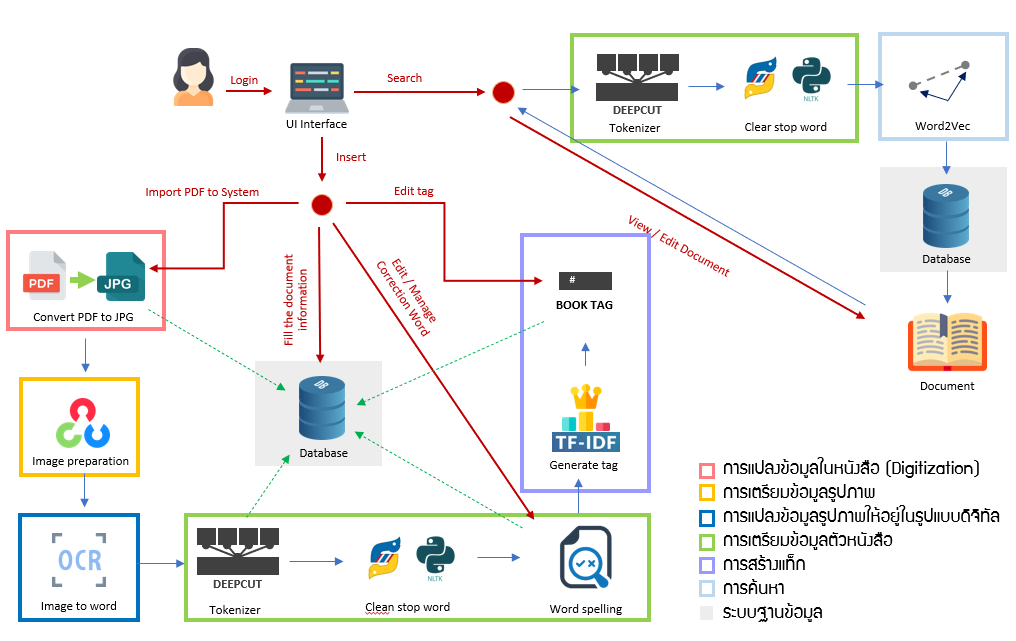
\includegraphics{systemoverview}
    \caption{System Overview}\label{fig:systemoverview}
\end{figure}

\section{Feature lists}
\subsection{การแปลงเอกสารเป็นรูปภาพ}

สำหรับการแปลงเอกสารผู้ใช้จะต้องทำการอัปโหลดไฟล์ PDF ของเอกสารเข้าสู่ระบบหลังจากนั้นจะระบบจะทำการแปลงแต่ละหน้าเป็นรูปภาพ JPG เพื่อนำไปใช้ต่อในขั้นต่อไปและนำใช้แสดงภายใน web application

\subsection{Image preparation}

ในส่วนของการจัดการรูปก่อนที่จะทำการ OCR ซึ่งรูปภาพนำมา OCR นั้นมาจากการสแกนทำให้ภาพส่วนใหญ่อยู่ในสภาพดีแต่ก็ยังคงมี noise  และมีความผิดพลาดจากการสแกนเช่น ภาพเอียง หรือตัวหนังสือไม่ชัดเกิดจากการขยับในระหว่างการสแกน หรือมีพื้นหลังสีที่ทำให้ OCR ไม่มีประสิทธิภาพ ดังนั้นจึงต้องมีการทำ Image processing ก่อนที่จะผ่านไปทำ OCR
ซึ่งในการทำ Image processing นั้นทางคณะผู้จัดทำได้ออกแบบไว้ว่าจะทำการแยกระหว่างรูปและตัวหนังสือออกจากกัน โดยการใช้ contour เข้ามาช่วยในการคัดแยกรูปออกจากตัวอักษร โดยดูจากพื้นที่สี่เหลี่ยมที่ได้จาก contour กลับพื้นที่ contour ว่ามีความต่างขนาดและความแตกต่างกันมากเท่าไร หรือใช้ขนาดความกว้างและยาวมาดูว่ามีขนาดเกินเท่าไรถึงจะตัดให้เป็นรูปภาพ
นอกจากนี้ออกแบบการหมุนโดยสร้าง contour บรรทัดและวัดความเอียงของแต่ละบรรทัดว่าเอียงเท่าไรจากนั้นจึงหมุนกลับในองศาตรงข้าม


\subsection{Image to word}

สำหรับการทำแปลงเอกสารเป็นข้อมูลดิจิตอลจะใช้ Tesseract OCR โดยจะใช้รูปภาพที่ผ่านกระบวนการ Image processing และประโยคที่แปลงออกมาได้จัดเก็บไว้ใช้งานต่อไป

\subsection{Text preprocessing}

สำหรับการทำ Text preprocessing จะประกอบไปด้วยการทำ Tokenizer หรือก็คือการตัดคำออกมาจากประโยคโดยการใช้อัลกอริทึม DeepCut และนำคำไปทำ Lemmatization หรือก็คือการลดรูปให้อยู่ในรูปแบบพื้นฐานของคำศัพท์เฉพาะภาษาอังกฤษโดยใช้ library nltk เป็นตัวจัดการก่อนจะนำไปลบ stop word คือการลบคำที่ไม่มีความหมายออกไปโดยใช้กลุ่มข้อมูลของ library pythianlp ก่อนนำไปตรวจสอบคำผิดก่อนโดยใช้อัลกอริทึมของ pythianlp และตรวจเช็คคำเฉพาะที่คณะผู้จัดทำได้กำหนดไว้โดยใช้ Minimum edit distance ก่อนที่จะนำไปใช้งานต่อไป

\subsection{Tag generated}

หลังจากที่นำข้อมูลที่ได้จากการทำ OCR และทำการเตรียมข้อมูลเสร็จเรียบร้อยแล้ว ระบบจะทำการคืนคำแต่ละหน้าให้กับผู้ใช้เพื่อที่จะให้ผู้ใช้สามารถเช็คคำที่ระบบอ่าน และแก้ไขคำเหล่านี้ได้ หลังจากนั้นเมื่อผู้ใช้เช็คคำเสร็จแล้ว ระบบจะนำคำทั้งหมดที่ได้ไปคิดคำนวณเพื่อทำการสร้างคะแนนให้แต่ละคำและทำการจัดลำดับคะแนนให้กับหนังสือเล่มนั้น ๆ โดยใช้การคิดคะแนนด้วยอัลกอริทึม TF-IDF 

\subsection{Search}

ในส่วนของระบบการค้นหานั้นเมื่อผู้ใช้ทำการกรอกคำค้นหาระบบจะทำการนำคำที่ผู้ใช้กรอกมาทำ Text preprocessing อีกครั้งหนึ่งแต่จะไม่ทำในส่วนของการตรวจเช็คคำ ผิด และคำที่ได้จะถูกนำไปเข้าโมเดล Word2Vec เพื่อนำไปค้นหาคำใกล้เคียงของคำค้นหาก่อนที่จะนำคำที่ได้ไปค้นในฐานข้อมูลเพื่อค้นหาหนังสือที่มีความใกล้เคียงกับคำค้นหามากที่สุด เมื่อได้หนังสือมาระบบจะทำการส่งข้อมูลหนังสือกลับไปให้ผู้ใช้

\subsection{Manage Book}

ในการจัดการข้อมูลเอกสารภายในระบบจะแบ่งทั้ง 3 ส่วนนั้นคือ 1. การเพิ่มเอกสารเข้าสู่ระบบ 2.การแก้ไขเอกสารภายในระบบ  3. การลบเอกสารออกจากระบบ 
ส่วนที่ 1. ในการเพิ่มเอกสารเข้าสู่ระบบ ผู้ใช้งานจะต้องอัปโหลดไฟล์เอกสารในรูปแบบ PDF และกรอกรายละเอียดของเอกสารเพื่อเข้าสู่กระบวนการแปลงเอกสารเป็นรูปภาพต่อไปจะเป็นการทำ Image processing ก่อนที่จะนำมาทำการแปลงภาพเป็นตัวอักษรเพื่อที่จะได้ข้อมูลดิจิตอลจากเอกสารที่ผู้ใช้เพิ่มเข้าสู่ระบบหลังจากนั้นจะเป็นการทำ Text preprocessing และให้ผู้ใช้งานได้ตรวจสอบคำอีกนึงครั้งก่อนที่นำคำเหล่านี้ไปผ่านกระบวนการ tag generate เพื่อหาคำสำคัญในเอกสารโดยให้ผู้ใช้งานได้ตรวจสอบแก้ไขหรือเพิ่มเติมก่อนจะสิ้นสุดการเพิ่มเอกสารเข้าสู่ระบบ ในส่วนที่ 2 การแก้ไขเอกสารภายในระบบผู้ใช้งานสามารถค้นหาเอกสารภายในระบบเพื่อนำมาแก้ไขรายละเอียดที่ผู้ใช้งานกรอกเท่านั้นแต่มาสามารถแก้ไขคำที่ถูกแปลงออกมาเป็นดิจิตอลอีกครั้งได้ และส่วนสุดท้ายการลบเอกสารในระบบผู้ใช้งานสามารถลบเอกสารภายในระบบได้โดยการค้นหาเอกสารที่ต้องการและกดลบเอกสารนั้นออกจากระบบโดยเมื่อมีการลบเอกสารออกก็จะลบคำที่มีอยู่ในเอกสารออกไปจากระบบเช่นกัน

\subsection{Login}

ผู้ใช้งานสามารถเข้าสู่ระบบเพื่อใช้งานฟังก์ชั่นต่าง ๆภายในระบบโดยเมื่อผู้ใช้งานทำการเข้าสู่ระบบด้วยชื่อผู้ใช้งานและรหัสผ่านแล้วจะได้รับ “token” เพื่อที่จะใช้สำหรับการยืนยันตัวในการใช้ฟังก์ชั่นต่าง ๆภายในระบบและผู้ใช้งานจะสามารถออกจากระบบได้

\section{System requirements}

\underline{ฝั่งผู้ใช้งาน}

ใช้งานได้บนระบบ web browser 

\begin{itemize}
    \item Google Chrome เวอร์ชั่น 84.0 ขึ้นไป 
    \item Microsoft Edge เวอร์ชั่น 83.0 ขึ้นไป
    \item Firefox เวอร์ชั่น 75.0 ขึ้นไป
\end{itemize}
 
\underline{ฝั่งเซิร์ฟเวอร์}
		
ทางด้าน Hardware

        \begin{itemize}
            \item CPU: Intel or AMD processor with 64-bit โดยที่ต้องมี 2 Core ขึ้นไป
            \item GPU: NVIDIA 1050ti or higher
            \item Disk Storage: 10 GB
            \item RAM: 8GB or higher
        \end{itemize}
        
		ทางด้าน Software แบ่งเป็น 2 ส่วนคือ Python และ JavaScript 
        \begin{enumerate}
            \item Python Backend
            \begin{itemize}
                \item Python เวอร์ชั่น 3.7.5
		        \item Tensorflow เวอร์ชั่น 2.3.1
		        \item DeepCut เวอร์ชั่น 0.7
		        \item Django เวอร์ชั่น 3.1.3
		        \item Djangorestframework เวอร์ชั่น 3.12.2
		        \item Django-cors-headers เวอร์ชั่น 3.5.0
		        \item Pythainlp เวอร์ชั่น 2.2.5
		        \item Pyspellchecker เวอร์ชั่น 0.5.5
		        \item nltk เวอร์ชั่น 3.5.0
		        \item mysqlclient เวอร์ชั่น 2.0.1
		        \item pillow เวอร์ชั่น 8.0.1
		        \item shapely เวอร์ชั่น 1.7.1
		        \item pytesseract เวอร์ชั่น 5.0.0 beta
		        \item opencv-python เวอร์ชั่น 4.4.0.46
		        \item pdf2image เวอร์ชั่น 1.14.0
		        \item scipy เวอร์ชั่น 1.5.4
            \end{itemize}
            \item JavaScript Backend and Frontend
		    \begin{itemize}
                \item nodejs เวอร์ชั่น 12.16.3
		        \item apollo-server-express เวอร์ชั่น 2.19.0
		        \item axios เวอร์ชั่น 0.20.0
		        \item cors เวอร์ชั่น 2.8.5
 		        \item dotenv เวอร์ชั่น 8.2.0
		        \item express เวอร์ชั่น 4.17.1
		        \item graphql เวอร์ชั่น 15.4.0
		        \item jsonwebtoken เวอร์ชั่น 8.5.1
		        \item knex เวอร์ชั่น 0.21.5
		        \item morgan เวอร์ชั่น 1.10.0
		        \item mysql2 เวอร์ชั่น 2.2.1
		        \item password-hash เวอร์ชั่น 1.2.2
		        \item react เวอร์ชั่น 16.13.1
		        \item react-hook-form เวอร์ชั่น 6.3.1
		        \item react-router-dom เวอร์ชั่น 5.2.0
		        \item styled-components เวอร์ชั่น 5.1.1
		        \item props-types เวอร์ชั่น 15.7.2
            \end{itemize}
        \end{enumerate}
		
\section{Database Design}

\begin{figure}[H]
    \centering
    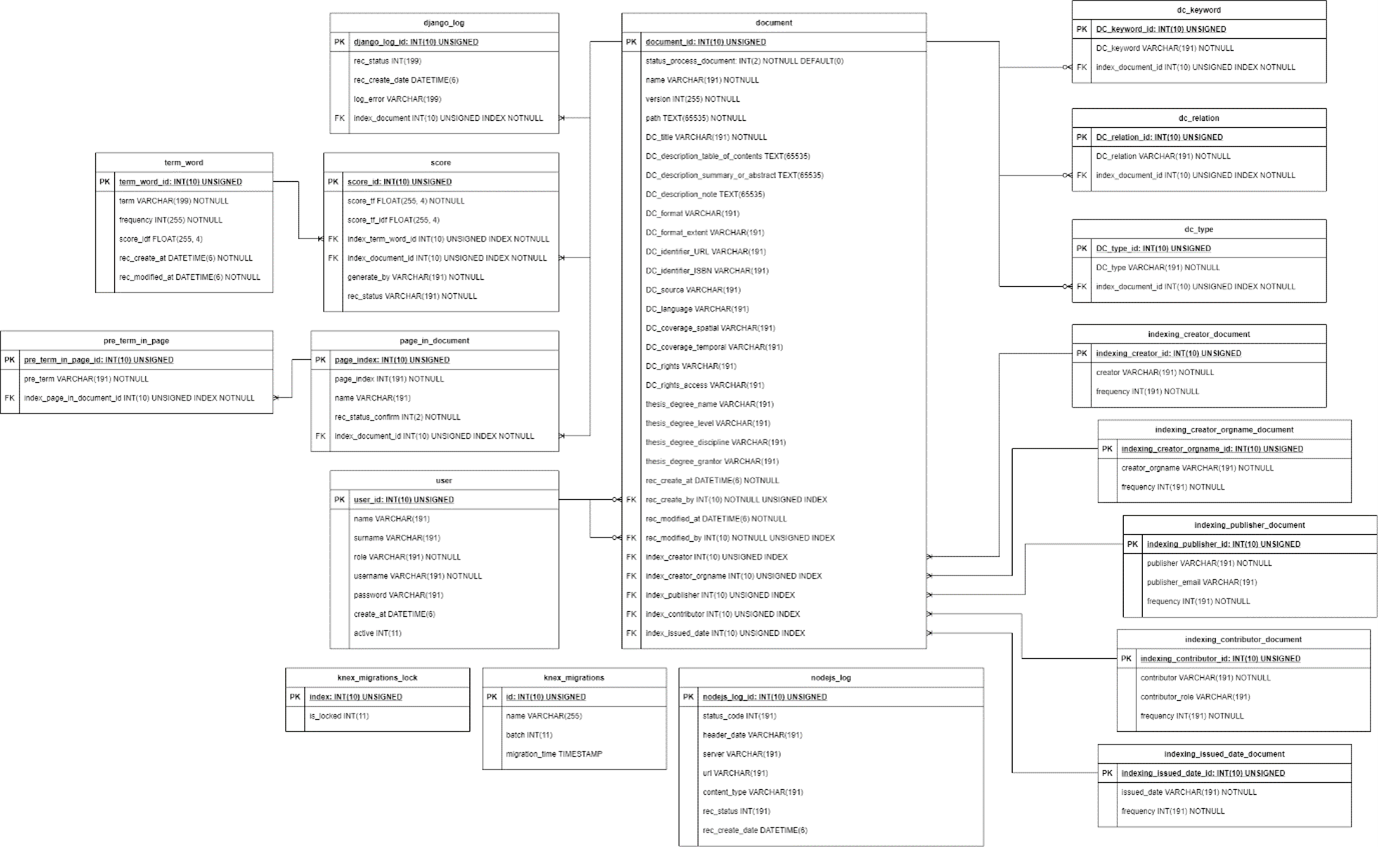
\includegraphics{er}
    \caption{แสดง ER Diagram ของฐานข้อมูล}\label{fig:er}
\end{figure}


\begin{figure}[H]
    \centering
    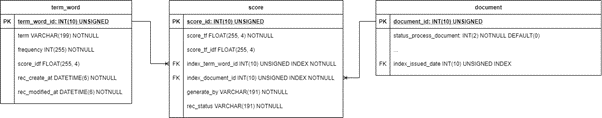
\includegraphics{er1}
    \caption{แสดง ER Diagram ส่วนของการเก็บความผิดพลาดในการสร้างคีย์เวิร์ดจากเอกสาร}\label{fig:er1}
\end{figure}


\begin{figure}[H]
    \centering
    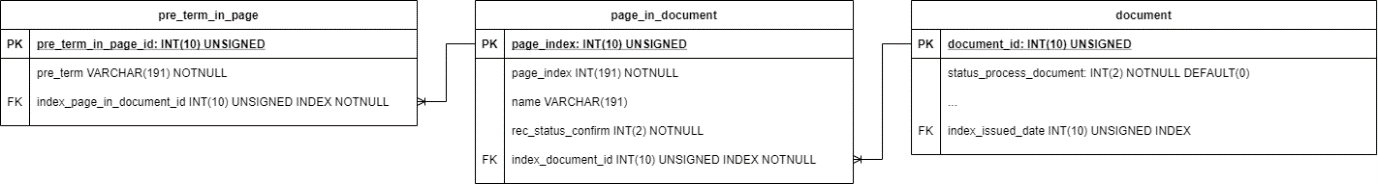
\includegraphics{er2}
    \caption{แสดง ER Diagram ส่วนของคีย์เวิร์ดและคะแนนความสำคัญในระบบ}\label{fig:er2}
\end{figure}


\begin{figure}[H]
    \centering
    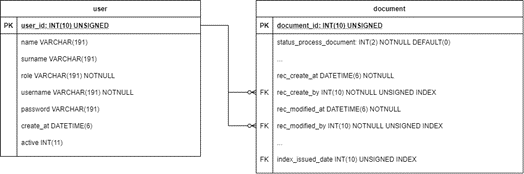
\includegraphics{er3}
    \caption{แสดง ER Diagram ส่วนของการเก็บคำจากแต่ละหน้าที่แปลงมาจากเอกสาร}\label{fig:er3}
\end{figure}


\begin{figure}[H]
    \centering
    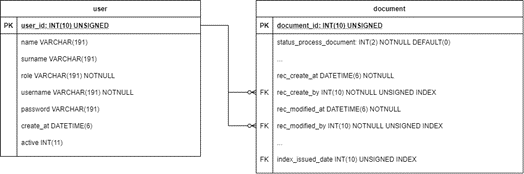
\includegraphics{er4}
    \caption{แสดง ER Diagram ส่วนของประวัติของผู้ใช้งานมีการสร้างหรือแก้ไขเอกสาร}\label{fig:er4}
\end{figure}



\begin{figure}[H]
    \centering
    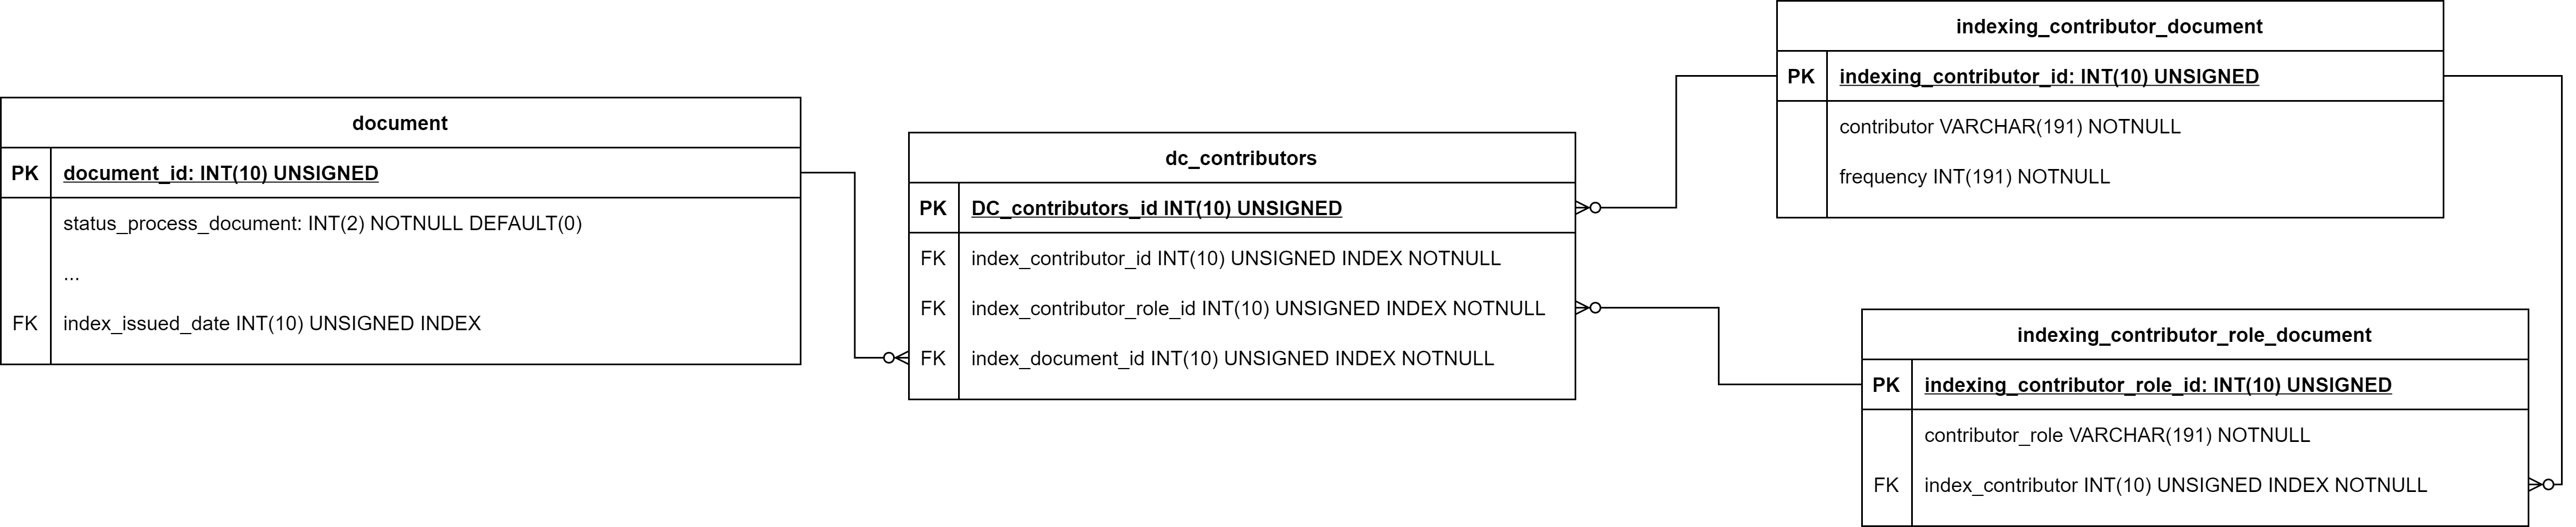
\includegraphics{er5}
    \caption{แสดง ER Diagram ส่วนของการเก็บข้อมูล keyword, relation, type ของเอกสาร}\label{fig:er5}
\end{figure}



\begin{figure}[H]
    \centering
    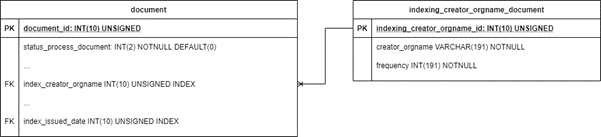
\includegraphics{er6}
    \caption{แสดง ER Diagram ส่วนของ Creator มีความเกี่ยวข้องกับเอกสารไหนบ้าง}\label{fig:er6}
\end{figure}



\begin{figure}[H]
    \centering
    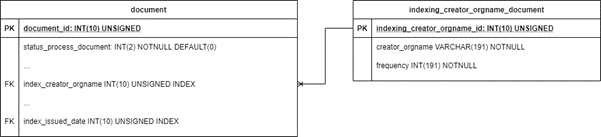
\includegraphics{er7}
    \caption{แสดง ER Diagram ส่วนของ Creator Organized Name มีความเกี่ยวข้องกับเอกสารไหนบ้าง}\label{fig:er7}
\end{figure}



\begin{figure}[H]
    \centering
    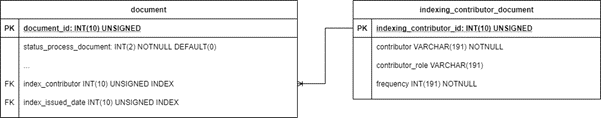
\includegraphics{er8}
    \caption{แสดง ER Diagram ส่วนของ Publisher มีความเกี่ยวข้องกับเอกสารไหนบ้าง}\label{fig:er8}
\end{figure}



\begin{figure}[H]
    \centering
    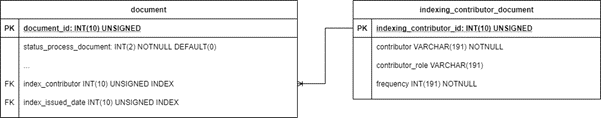
\includegraphics{er9}
    \caption{แสดง ER Diagram ส่วนของ Contributor มีความเกี่ยวข้องกับเอกสารไหนบ้าง}\label{fig:er9}
\end{figure}



\begin{figure}[H]
    \centering
    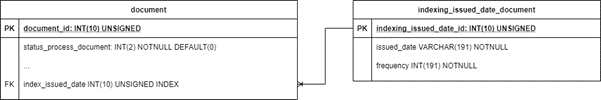
\includegraphics{er10}
    \caption{แสดง ER Diagram ส่วนของ Issued Date มีความเกี่ยวข้องกับเอกสารไหนบ้าง}\label{fig:er10}
\end{figure}



\begin{figure}[H]
    \centering
    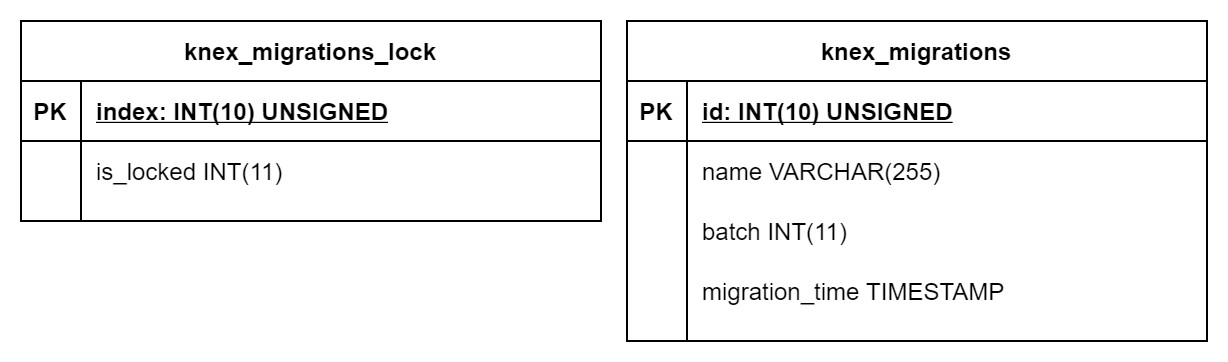
\includegraphics{er11}
    \caption{แสดง ER Diagram ส่วนของ Knex module ที่ใช้สำหรับ Migration ฐานข้อมูล}\label{fig:er11}
\end{figure}



\begin{figure}[H]
    \centering
    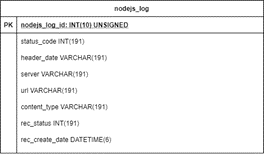
\includegraphics{er12}
    \caption{แสดง ER Diagram ส่วนของการเก็บประวัติการ HTTP Request NodeJS ไปยัง Django}\label{fig:er12}
\end{figure}

\subsection{Database Structure}
รูปที่ 3.2 แสดงฐานข้อมูลของทั้งระบบโดยจะมีหลัก ๆ ทั้งหมดสามส่วน ทางด้านฝั่งขวาของตาราง document จะเป็นตารางที่เก็บข้อมูลเพิ่มเติมจากตาราง document และส่วนทางด้านฝั่งซ้ายของตาราง document สำหรับการเก็บข้อมูลในด้านของการทำระบบการเก็บคำจากเอกสารที่ถูกใส่ลงมาในระบบ ระบบการแปลงคำเป็นคีย์เวิร์ดและคะแนน TF-IDF ที่นำมาใช้สำหรับการค้นหาเอกสาร ระบบจัดการฐานข้อมูลผู้ใช้งาน และการตรวจสอบความผิดพลาดที่มีโอกาสจากการสร้างคีย์เวิร์ด และส่วนสุดท้ายที่เป็นตารางที่ไม่มีการเชื่อมโยงกับตารางใด ๆ จะมีไว้สำหรับการทำระบบฐานข้อมูล และระบบตรวจสอบ HTTP Request ของทาง NodeJS

รูปที่ 3.3 จะเป็นส่วนของการเก็บข้อผิดพลาดที่มาจากระหว่างการสร้างคีย์เวิร์ด และการสร้างคะแนน Term-Frequency  โดยในส่วนนี้มีตาราง document ที่มีความสัมพันธ์ 1 to many กับตาราง django\_log กล่าวก็คือในหนึ่งเอกสารมีได้หลายบันทึกของ Django เนื่องมีโอกาสที่เกิดความผิดพลาดแล้วต้องทำใหม่จนกว่าจะไม่มีความผิดพลาดเกิดขึ้น

รูปที่ 3.4 จะเป็นส่วนของคีย์เวิร์ด และคะแนนเพื่อนำมาใช้สำหรับการค้นหาเอกสารของระบบนี้ โดยจะมีทั้งหมดสามตาราง document, term\_word, score ตาราง document จะเป็นตารางที่เก็บข้อมูลของเอกสารไว้ ส่วนตาราง term\_word จะเป็นการเก็บคีย์เวิร์ด และคะแนน IDF สำหรับการลดความสำคัญของคีย์เวิร์ดนั้น ๆ ไว้ซึ่งทั้งสองตารางนี้จะเป็นความสัมพันธ์แบบ one to many กับตาราง score ที่จะมีคะแนนสำหรับระบบการค้นหาเก็บเอาไว้ ที่มีความสัมพันธ์แบบนี้เนื่องจากในแต่ละคีย์เวิร์ดมีโอกาสพบได้ในหลายเอกสาร และเอกสารเองก็สามารถมีได้หลายคีย์เวิร์ด เนื่องจากแต่ละคีย์เวิร์ดที่อยู่ต่างเอกสารกันจะมีคะแนนไม่เท่ากัน

รูปที่ 3.5 จะเป็นส่วนของการเก็บคำที่แปลงมาจากเอกสารไว้โดยเริ่มที่ตาราง document จะที่สามารถบอกได้ว่าเอกสารไหน ที่จะมีความพันธ์ one to many ไปยังตาราง page\_in\_document ที่จะเป็นตารางที่บอกถึงหน้าต่าง ๆ ในเอกสารนั้น และยังมีความสัมพันธ์ one to many ต่อไปยังตาราง per\_term\_in\_page ที่จะมีคำต่าง ๆ เก็บเอาไว้ ดังนั้นจะเป็นความสัมพันธ์ที่เอกสารนั้นจะสามารถมีได้หลายหน้า แล้วแต่ละหน้าเองก็จะมีคำต่าง ๆ ที่แปลงออกมาถูกเก็บเอาไว้

รูปที่ 3.6 จะเป็นความสัมพันธ์ของบัญชีผู้ใช้กับเอกสาร โดยจะมีตาราง user ที่จะเก็บข้อมูลของผู้ใช้งานที่มีความสัมพันธ์แบบ one to many ไปยังตาราง document ที่จะเก็บต้องเก็บข้อมูลของผู้ใช้ไว้ว่าผู้ใช้คนไหนเป็นคนสร้าง หรือแก้ไขเอกสารนี้ ซึ่งบัญชีผู้ใช้สามารถสร้างหรือแก้ไขเอกสารได้หลายเอกสาร

รูปที่ 3.7 จะเป็นส่วนของข้อมูลของตาราง Document เหมือนกันแต่เนื่องจากข้อมูลมีมากกว่าหนึ่งทำให้ต้องสร้างความสัมพันธ์แบบ one to many กับตาราง dc\_keyword, dc\_relation, dc\_type ซึ่งจะเป็นข้อมูลคีย์เวิร์ด ความสัมพันธ์ และประเภทของเอกสารตามลำดับ

รูปที่ 3.8 จะเป็นส่วนของการเก็บความสัมพันธ์ระหว่าง Creator กับเอกสาร เนื่องจาก Creator สามารถมีได้หลายเอกสารทำให้ตาราง indexing\_creator\_document จะเป็นความสัมพันธ์แบบ one to many กับตาราง document 

รูปที่ 3.9 จะเป็นส่วนของการเก็บความสัมพันธ์ระหว่าง Creator orgname กับเอกสารเนื่อง จากCreator orgname สามารถมีได้หลายเอกสารทำให้ตาราง indexing\_creator\_orgname\_document จะเป็นความสัมพันธ์แบบ one to many กับตาราง document 

รูปที่ 3.10 จะเป็นส่วนของการเก็บความสัมพันธ์ระหว่าง Publisher กับเอกสาร เนื่องจาก Publisher สามารถมีได้หลายเอกสารทำให้ตาราง indexing\_publisher\_document จะเป็นความสัมพันธ์แบบ one to many กับตาราง document 

รูปที่ 3.11 จะเป็นส่วนของการเก็บความสัมพันธ์ระหว่าง Contributor กับเอกสาร เนื่องจาก Contributor สามารถมีได้หลายเอกสารทำให้ตาราง Indexing\_contributor\_document จะเป็นความสัมพันธ์แบบ one to many กับตาราง document 

รูปที่ 3.12 จะเป็นส่วนของการเก็บความสัมพันธ์ระหว่าง Issued Date กับเอกสาร เนื่องจาก Issued Date สามารถมีได้หลายเอกสารทำให้ตาราง indexing\_issued\_date\_document จะเป็นความสัมพันธ์แบบ one to many กับตาราง document 

รูปที่ 3.13 จะเป็นสองตารางที่บันทึกการจัดการฐานข้อมูลของเครื่องมือที่ชื่อว่า Knex ที่จะทำการจัดการสร้างฐานข้อมูล ด้วยคำสั่ง Migration แล้วหลังจากทำคำสั่งเสร็จสิ้นจะเก็บบันทึกไว้

รูปที่ 3.14 จะเป็นตารางสำหรับการเก็บ HTTP Request จาก NodeJS ที่ส่งไปทางฝั่งของ Django ซึ่งจะถูกเก็บข้อมูลไว้ในตารางนี้

\subsection{Database Dictionary}

อธิบายถึงชื่อของคอลัมน์ ความหมายและลักษณะการเก็บข้อมูลภายในฐานข้อมูลโดยที่ตารางมีทั้งหมด 18 ตารางดังนี้



\begin{table}[H]
\caption{ตารางอธิบายความหมายตาราง term\_word}\label{tbl:termword}
\begin{tabular}{|l|l|l|}
\hline
\multicolumn{1}{|c|}{ชื่อคอลัมน์} & \multicolumn{1}{c|}{ความหมาย}             & \multicolumn{1}{c|}{ประเภท}                          \\ \hline
term\_word\_id    & id   สำหรับบ่งบอกคำศัพท์                 & \makecell[l]{INT   (10) PK\\ Auto\_Increment}     \\ \hline
term              & คำศัพท์                                  & VARCHAR   (191)                                                                   \\ \hline
frequency         & จำนวนความถี่ของเอกสารที่มีคำศัพท์นี้อยู่ & INT   (191)                                                                       \\ \hline
score\_idf        & คะแนน   idf ของคำศัพท์นี้                & FLOAT   (255,4)                                                                   \\ \hline
rec\_create\_at   & วันเวลาของการเพิ่มคำศัพท์นี้เข้าสู่ระบบ  & \makecell[l]{DATETIME   (6)\\   current\_timestamp} \\ \hline
rec\_modified\_at & วันเวลาที่อัปเดทข้อมูลของคำศัพท์         & \makecell[l]{DATETIME   (6)\\  current\_timestamp} \\ \hline
\end{tabular}
\end{table}

\begin{table}[H]
\caption{ตารางอธิบายความหมายตาราง user}\label{tbl:user}
\begin{tabular}{|l|l|l|}
\hline
\multicolumn{1}{|c|}{ชื่อคอลัมน์} & \multicolumn{1}{c|}{ความหมาย}             & \multicolumn{1}{c|}{ประเภท}                                     \\ \hline
user\_id                          & id   สำหรับบ่งบอกผู้ใช้งาน                & \makecell[l]{INT   (10) PK\\    Auto\_Increment}     \\ \hline
name                              & ชื่อของผู้ใช้งาน                          & VARCHAR   (50)                                                                    \\ \hline
surname                           & นามสกุลของผู้ใช้งาน                       & VARCHAR   (191)                                                                   \\ \hline
role                              & ตำแหน่งของผู้ใช้งาน                       & VARCHAR   (191)                                                                   \\ \hline
username                          & ชื่อผู้ใช้งานสำหรับทำการ   login          & VARCHAR   (191)                                                                   \\ \hline
password                          & รหัสผ่านผู้ใช้งานสำหรับทำการ   login      & VARCHAR   (191)                                                                   \\ \hline
create\_at                        & วันเวลาของผู้ใช้งานของการเพิ่มเข้าสู่ระบบ & \makecell[l]{DATETIME   (6) \\ current\_timestamp} \\ \hline
active                            & สถานะการระงับบัญชีผู้ใช้งาน               & \makecell[l]{INT   (11) \\ Default 1}             \\ \hline
\end{tabular}
\end{table}

\begin{table}[H]
\caption{ตารางอธิบายความหมายตาราง score}\label{tbl:score}        
\begin{tabular}{|l|l|l|}
\hline
\multicolumn{1}{|c|}{ชื่อคอลัมน์} & \multicolumn{1}{c|}{ความหมาย}                                      & \multicolumn{1}{c|}{ประเภท}                                                   \\ \hline
score\_id             & id   สำหรับบ่งบอกคะแนนของคำศัพท์ &\makecell[l]{INT   (10) PK\\    \\ Auto\_Increment}      \\ \hline
score\_tf             & คะแนน   tf ของคำศัพท์            & FLOAT   (255,4)                                                                     \\ \hline
score\_tf\_idf        & คะแนน   tf-idf ของคำศัพท์        & FLOAT   (255,4)                                                                     \\ \hline
index\_term\_word\_id & id   สำหรับบ่งบอกคำศัพท์         & INT   (10)                                                                          \\ \hline
index\_document\_id   & id สำหรับบ่งบอกเอกสาร            & INT   (10)                                                                          \\ \hline
generate\_by          & คะแนนถูกคำนวณโดยใคร              &\makecell[l]{VARCHAR   (191)\\    \\ Default   ‘default’}\\ \hline
rec\_status           & สถานะการใช้คะแนนนี้              &\makecell[l]{INT   (191)\\    \\ Default 1}              \\ \hline
\end{tabular}
\end{table}

\begin{table}[H]
\caption{ตารางอธิบายความหมายตาราง pre\_term\_in\_page}\label{tbl:preterminpage}        
\begin{tabular}{|l|l|l|}
\hline
\multicolumn{1}{|c|}{ชื่อคอลัมน์} & \multicolumn{1}{c|}{ความหมาย}                                      & \multicolumn{1}{c|}{ประเภท}                                                   \\ \hline
pre\_term\_in\_page\_id           & id   สำหรับบ่งบอกคำศัพท์ชั่วคราวที่รอให้ผู้ใช้งานตรวจสอบ           & \makecell[l]{INT   (10) PK\\Auto\_Increment} \\ \hline
pre\_term                         & คำศัพท์ชั่วคราวที่รอให้ผู้ใช้ตรวจสอบ                               & VARCHAR   (191)                                                               \\ \hline
index\_page\_in\_document\_id     & id   สำหรับบ่งบอกที่อยู่ของคำศัพท์ชั่วคราวที่รอให้ผู้ใช้งานตรวจสอบ & INT (10) FK                                                                   \\ \hline
\end{tabular}
\end{table}

\begin{table}[H]
\caption{ตารางอธิบายความหมายตาราง page\_in\_document}\label{tbl:pageindocument}        
\begin{tabular}{|l|l|l|}
\hline
\multicolumn{1}{|c|}{ชื่อคอลัมน์} & \multicolumn{1}{c|}{ความหมาย}                                      & \multicolumn{1}{c|}{ประเภท}                                                   \\ \hline
page\_in\_document\_id            & id   สำหรับบ่งบอกที่อยู่ของคำศัพท์ชั่วคราวที่รอให้ผู้ใช้งานตรวจสอบ & \makecell[l]{INT   (10) PK\\Auto\_Increment} \\ \hline
page\_index                       & หน้าของเอกสาร                                                      & INT   (191)                                                                   \\ \hline
name                              & ชื่อ   File ของข้อมูล                                              & VARCHAR   (191)                                                               \\ \hline
rec\_status\_confirm              & สถานะการยืนยันโดยผู้ใช้งาน                                         & \makecell[l]{INT   (2)\\Default   2}         \\ \hline
index\_document\_id               & id สำหรับบ่งบอกเอกสาร                                              & INT (10) FK                                                                   \\ \hline
\end{tabular}
\end{table}

\begin{table}[H]
\caption{ตารางอธิบายความหมายตาราง nodejs\_log}\label{tbl:nodejslog}        
\begin{tabular}{|l|l|l|}
\hline
\multicolumn{1}{|c|}{ชื่อคอลัมน์} & \multicolumn{1}{c|}{ความหมาย}                     & \multicolumn{1}{c|}{ประเภท}                                                       \\ \hline
nodejs\_log\_id                   & id สำหรับการจัดเก็บประวัติการทำงานฝั่ง nodejs     & \makecell[l]{INT   (10) PK \\ Auto\_Increment}    \\ \hline
status\_code                      & เก็บสถานะ   HTTP หลังจากที่ส่งไปแล้วว่าได้สถานะใด & INT   (191)                                                                       \\ \hline
header\_date                      & เก็บข้อมูล   header ของ HTTP ที่ส่งไป             & VARCHAR   (191)                                                                   \\ \hline
server                            & ชื่อรูปแบบของเซิฟเวอร์ที่ส่งไป                    & VARCHAR   (191)                                                                   \\ \hline
url                               & ตำแหน่งโดเมนหรือ   IP ที่ส่งไป                    & INT   (10) FK                                                                     \\ \hline
content\_type                     & รูปแบบเนื้อหาที่ส่งไป                             & VARCHAR   (191)                                                                   \\ \hline
rec\_status                       & สถานะที่บอกว่าการส่งเกิดข้อผิดพลาดระหว่างทาง      & INT   (191)                                                                       \\ \hline
rec\_create\_date                 & วันเวลาที่ทำการส่ง   ณ ตอนนั้น                    & \makecell[l]{DATETIME   (6) \\ current\_timestamp}\\ \hline
\end{tabular}
\end{table}

\begin{table}[H]
\caption{ตารางอธิบายความหมายตาราง knex\_migrations\_lock}\label{tbl:knexmigrationslock}        
\begin{tabular}{|l|l|l|}
\hline
\multicolumn{1}{|c|}{ชื่อคอลัมน์} & \multicolumn{1}{c|}{ความหมาย}              & \multicolumn{1}{c|}{ประเภท}                                                   \\ \hline
index                             & id   บ่งบอกลำดับของไฟล์ migration ของ knex & \makecell[l]{INT   (10) PK\\Auto\_Increment} \\ \hline
is\_locked                        & สถานะของไฟล์   migration                   & INT (11)                                                                      \\ \hline
\end{tabular}
\end{table}

\begin{table}[H]
\caption{ตารางอธิบายความหมายตาราง knex\_migrations}\label{tbl:knexmigrations}        
\begin{tabular}{|l|l|l|}
\hline
\multicolumn{1}{|c|}{ชื่อคอลัมน์} & \multicolumn{1}{c|}{ความหมาย}                      & \multicolumn{1}{c|}{ประเภท}                                                   \\ \hline
id                                & id   บ่งบอกลำดับการทำงานของไฟล์ migration ของ knex & \makecell[l]{INT   (10) PK\\Auto\_Increment} \\ \hline
name                              & ชื่อไฟล์   migration ที่ถูกทำงานเรียบร้อย          & VARCHAR   (255)                                                               \\ \hline
batch                             & ลำดับที่                                           & INT   (11)                                                                    \\ \hline
migration\_time                   & เวลาที่ถุกสั่งให้ทำงาน                             & \makecell[l]{TIMESTAMP\\current\_timestamp}  \\ \hline
\end{tabular}
\end{table}

\begin{table}[H]
\caption{ตารางอธิบายความหมายตาราง indexing\_publisher\_document}\label{tbl:indexingpublisherdocument}        
\begin{tabular}{|l|l|l|}
\hline
\multicolumn{1}{|c|}{ชื่อคอลัมน์} & \multicolumn{1}{c|}{ความหมาย}      & \multicolumn{1}{c|}{ประเภท}                                                   \\ \hline
indexing\_publisher\_id           & id สำหรับบ่งบอกสำนักพิมพ์          & \makecell[l]{INT   (10) PK\\Auto\_Increment} \\ \hline
publisher                         & ชื่อสำนักพิมพ์                     & VARCHAR   (191)                                                               \\ \hline
publisher\_email                  & e-mail   ของสำนักพิมพ์             & VARCHAR   (191)                                                               \\ \hline
frequency                         & จำนวนของสำนักพิมพ์นี้ที่ถูกอ้างอิง & INT (191)                                                                     \\ \hline
\end{tabular}
\end{table}

\begin{table}[H]
\caption{ตารางอธิบายความหมายตาราง indexing\_issued\_date\_document}\label{tbl:indexingissueddatedocument}        
\begin{tabular}{|l|l|l|}
\hline
\multicolumn{1}{|c|}{ชื่อคอลัมน์} & \multicolumn{1}{c|}{ความหมาย}             & \multicolumn{1}{c|}{ประเภท}                                                   \\ \hline
indexing\_issued\_date\_id        & id สำหรับบ่งบอกปีที่เขียน                 & \makecell[l]{INT   (10) PK\\Auto\_Increment} \\ \hline
issued\_date                      & วันเวลาของปีที่เขียนเอกสาร                & DATE                                                                          \\ \hline
frequency                         & จำนวนของวันเวลาของปีที่เขียนที่ถูกอ้างอิง & INT (191)                                                                     \\ \hline
\end{tabular}
\end{table}

\begin{table}[H]
\caption{ตารางอธิบายความหมายตาราง indexing\_creator\_orgname\_document}\label{tbl:indexingcreatororgnamedocument}        
\begin{tabular}{|l|l|l|}
\hline
\multicolumn{1}{|c|}{ชื่อคอลัมน์} & \multicolumn{1}{c|}{ความหมาย}                & \multicolumn{1}{c|}{ประเภท}                                                   \\ \hline
indexing\_creator\_orgname\_id    & id สำหรับบ่งบอกชื่อหน่วยงานรับผิดชอบสังกัด   & \makecell[l]{INT   (10) PK\\Auto\_Increment} \\ \hline
creator\_orgname                  & ชื่อหน่วยงานรับผิดชอบสังกัด                  & VARCHAR   (191)                                                               \\ \hline
frequency                         & จำนวนของหน่วยงานรับผิดชอบสังกัดที่ถูกอ้างอิง & INT (191)                                                                     \\ \hline
\end{tabular}
\end{table}

\begin{table}[H]
\caption{ตารางอธิบายความหมายตาราง indexing\_creator\_document}\label{tbl:indexingcreatordocument}
\begin{tabular}{|l|l|l|}
\hline
\multicolumn{1}{|c|}{ชื่อคอลัมน์} & \multicolumn{1}{c|}{ความหมาย}       & \multicolumn{1}{c|}{ประเภท}                                                   \\ \hline
indexing\_creator\_id             & id สำหรับบ่งบอกชื่อผู้เขียนเอกสาร   & \makecell[l]{INT   (10) PK\\Auto\_Increment} \\ \hline
creator                           & ชื่อของผู้เขียนเอกสาร               & VARCHAR   (191)                                                               \\ \hline
frequency                         & จำนวนของผู้เขียนเอกสารที่ถูกอ้างอิง & INT (191)                                                                     \\ \hline
\end{tabular}
\end{table}

\begin{table}[H]
\caption{ตารางอธิบายความหมายตาราง indexing\_contributor\_document}\label{tbl:indexingcontributordocument}
\begin{tabular}{|l|l|l|}
\hline
\multicolumn{1}{|c|}{ชื่อคอลัมน์} & \multicolumn{1}{c|}{ความหมาย}              & \multicolumn{1}{c|}{ประเภท}                                                   \\ \hline
indexing\_contributor\_id         & id สำหรับบ่งบอกชื่อหน่วยข้อมูลผู้ร่วมงาน   & \makecell[l]{INT   (10) PK\\Auto\_Increment} \\ \hline
contributor                       & ชื่อหน่วยข้อมูลผู้ร่วมงาน                  & VARCHAR   (191)                                                               \\ \hline
contributor\_role                 & ตำแหน่งของหน่วยข้อมูลผู้ร่วมงาน            & VARCHAR   (191)                                                               \\ \hline
frequency                         & จำนวนของหน่วยข้อมูลผู้ร่วมงานที่ถูกอ้างอิง & INT (191)                                                                     \\ \hline
\end{tabular}
\end{table}

\begin{table}
\caption{ตารางอธิบายความหมายตาราง document}\label{tbl:document}
\vspace*{-1.25em}
\end{table}
\begin{longtable}[l]{|l|l|l|}
\hline
\multicolumn{1}{|c|}{ชื่อคอลัมน์}      & \multicolumn{1}{c|}{ความหมาย}                    & \multicolumn{1}{c|}{ประเภท}                                                       \\ \hline \endhead
document\_id                           & id สำหรับบ่งบอกเอกสาร                            & \makecell[l]{INT   (10) PK\\Auto\_Increment}     \\ \hline
status\_process\_document              & สถานะการทำงานของเอกสาร                           & INT   (2)                                                                         \\ \hline
name                                   & ชื่อไฟล์   PDF เอกสาร                            & VARCHAR   (191)                                                                   \\ \hline
version                                & ครั้งที่ตีพิมพ์                                  & INT   (255)                                                                       \\ \hline
path                                   & ตำแหน่งไฟล์   PDF ที่ผู้ใช้งานอัปโหลดเข้าสู่ระบบ & TEXT                                                                              \\ \hline
DC\_title                              & ชื่อเอกสาร                                       & VARCHAR   (191)                                                                   \\ \hline
DC\_title\_alternative                 & ชื่อรองของเอกสาร                                 & VARCHAR   (191)                                                                   \\ \hline
DC\_description\_table\_of\_contents   & สาระสำคัญที่มาจากสารบัญ                          & TEXT                                                                              \\ \hline
DC\_description\_summary\_or\_abstract & บทสรุปสาระสำคัญของหนังสือแต่ละเล่ม               & TEXT                                                                              \\ \hline
DC\_description\_note                  & รายละเอียดทั่วไปของเอกสาร                        & TEXT                                                                              \\ \hline
DC\_format                             & รูปแบบข้อมูลที่ถูกจัดเก็บในระบบ                  & VARCHAR   (191)                                                                   \\ \hline
DC\_format\_extent                     & ขนาดของไฟล์เอกสาร                                & VARCHAR   (191)                                                                   \\ \hline
DC\_identifier\_URL                    & แหล่งที่มาของเอกสาร                              & VARCHAR   (191)                                                                   \\ \hline
DC\_identifier\_ISBN                   & เลขมาตราฐานสากลของเอกสาร                         & VARCHAR   (191)                                                                   \\ \hline
DC\_source                             & หน่วยข้อมูลต้นฉบับ                               & VARCHAR   (191)                                                                   \\ \hline
DC\_language                           & ภาษาของเอกสาร                                    & VARCHAR   (191)                                                                   \\ \hline
DC\_coverage\_spatial                  & สถานที่ของเอกสารที่เป็นเจ้าของ                   & VARCHAR   (191)                                                                   \\ \hline
DC\_coverage\_temporal                 & ช่วงเวลาในหน่วยปีของเอกสาร                       & VARCHAR   (191)                                                                   \\ \hline
DC\_rights                             & ระดับการเข้าถึงของข้อมูล                         & VARCHAR   (191)                                                                   \\ \hline
DC\_rights\_access                     & ตำแหน่งที่มีสิทธิ์ในการเข้าถึงข้อมูล             & VARCHAR   (191)                                                                   \\ \hline
thesis\_degree\_name                   & ชื่อเต็มของปริญญา                                & VARCHAR   (191)                                                                   \\ \hline
thesis\_degree\_level                  & ระดับของปริญญา                                   & VARCHAR   (191)                                                                   \\ \hline
thesis\_degree\_discipline             & สาขาวิชา                                         & VARCHAR   (191)                                                                   \\ \hline
thesis\_degree\_grantor                & มหาวิทยาลัย                                      & VARCHAR   (191)                                                                   \\ \hline
rec\_create\_at                        & วันเวลาของเอกสารที่ถูกนำเข้าสู่ระบบ              & \makecell[l]{DATETIME   (6)\\current\_timestamp} \\ \hline
rec\_create\_by                        & id   สำหรับบ่งบอกผู้ใช้งานที่นำเอกสารเข้าสู่ระบบ & INT   (10) FK                                                                     \\ \hline
rec\_modified\_at                      & วันเวลาของเอกสารที่ถูกแก้ไขข้อมูล                & \makecell[l]{DATETIME   (6)\\current\_timestamp} \\ \hline
rec\_modified\_by                      & id   สำหรับบ่งบอกผู้ใช้งานที่แก้ไขเอกสารในระบบ   & INT   (10) FK                                                                     \\ \hline
index\_creator                         & id สำหรับบ่งบอกชื่อผู้เขียนเอกสาร                & INT   (10) FK                                                                     \\ \hline
index\_creator\_orgname                & id สำหรับบ่งบอกชื่อหน่วยงานรับผิดชอบสังกัด       & INT   (10) FK                                                                     \\ \hline
index\_publisher                       & id สำหรับบ่งบอกสำนักพิมพ์                        & INT   (10) FK                                                                     \\ \hline
index\_contributor                     & id สำหรับบ่งบอกชื่อหน่วยข้อมูลผู้ร่วมงาน         & INT   (10) FK                                                                     \\ \hline
index\_issued\_date                    & id สำหรับบ่งบอกปีที่เขียน                        & INT (10) FK                                                                       \\ \hline
\end{longtable}

\begin{table}[H]
\caption{ตารางอธิบายความหมายตาราง django\_log}\label{tbl:djangolog}
\begin{tabular}{|l|l|l|}
\hline
\multicolumn{1}{|c|}{ชื่อคอลัมน์} & \multicolumn{1}{c|}{ความหมาย}                 & \multicolumn{1}{c|}{ประเภท}                                                       \\ \hline
django\_log\_id                   & id สำหรับการจัดเก็บประวัติการทำงานฝั่ง django & \makecell[l]{INT   (10) PK\\Auto\_Increment}    \\ \hline
rec\_status                       & สถานะการทำงานที่เกิดขึ้น                      & INT   (191)                                                                       \\ \hline
rec\_create\_date                 & วันเวลาของการทำงานที่เกิดขึ้น                 & \makecell[l]{DATETIME   (6)\\current\_timestamp}\\ \hline
log\_error                        & ข้อมูลข้อผิดพลาดที่เกิดขึ้น                   & VARCHAR   (191)                                                                   \\ \hline
index\_document                   & id สำหรับบ่งบอกเอกสารที่ทำงาน                 & INT (10) FK                                                                       \\ \hline
\end{tabular}
\end{table}

\begin{table}[H]
\caption{ตารางอธิบายความหมายตาราง dc\_type}\label{tbl:dctype}
\begin{tabular}{|l|l|l|}
\hline
\multicolumn{1}{|c|}{ชื่อคอลัมน์} & \multicolumn{1}{c|}{ความหมาย}  & \multicolumn{1}{c|}{ประเภท}                                                   \\ \hline
DC\_type\_id                      & id สำหรับบ่งบอกประเภทของเอกสาร & \makecell[l]{INT   (10) PK\\Auto\_Increment} \\ \hline
DC\_type                          & ประเภทของเอกสาร                & VARCHAR   (191)                                                               \\ \hline
index\_document\_id               & id สำหรับบ่งบอกเอกสาร          & INT (10)                                                                      \\ \hline
\end{tabular}
\end{table}

\begin{table}[H]
\caption{ตารางอธิบายความหมายตาราง dc\_relation}\label{tbl:dcrelation}
\begin{tabular}{|l|l|l|}
\hline
\multicolumn{1}{|c|}{ชื่อคอลัมน์} & \multicolumn{1}{c|}{ความหมาย}      & \multicolumn{1}{c|}{ประเภท}                                                   \\ \hline
DC\_relation\_id                  & id สำหรับบ่งบอกเอกสารที่เกี่ยวข้อง & \makecell[l]{INT   (10) PK\\Auto\_Increment} \\ \hline
DC\_relation                      & ชื่อเอกสารที่เกี่ยวข้อง            & VARCHAR   (191)                                                               \\ \hline
index\_document\_id               & id สำหรับบ่งบอกเอกสาร              & INT (10)                                                                      \\ \hline
\end{tabular}
\end{table}

\begin{table}[H]
\caption{ตารางอธิบายความหมายตาราง dc\_keyword}\label{tbl:dckeyword}
\begin{tabular}{|l|l|l|}
\hline
\multicolumn{1}{|c|}{ชื่อคอลัมน์} & \multicolumn{1}{c|}{ความหมาย}      & \multicolumn{1}{c|}{ประเภท}                                                   \\ \hline
DC\_keyword\_id                   & id สำหรับบ่งบอก tag           & \makecell[l]{INT   (10) PK\\Auto\_Increment} \\ \hline
DC\_keyword                       & คำศัพท์                       & VARCHAR   (191)                                                               \\ \hline
index\_document\_id               & id สำหรับบ่งบอกเอกสาร              & INT (10)                                                                      \\ \hline
\end{tabular}
\end{table}

\section{UML Design}
\subsection{Use case diagram}

\begin{figure}[H]
    \centering
    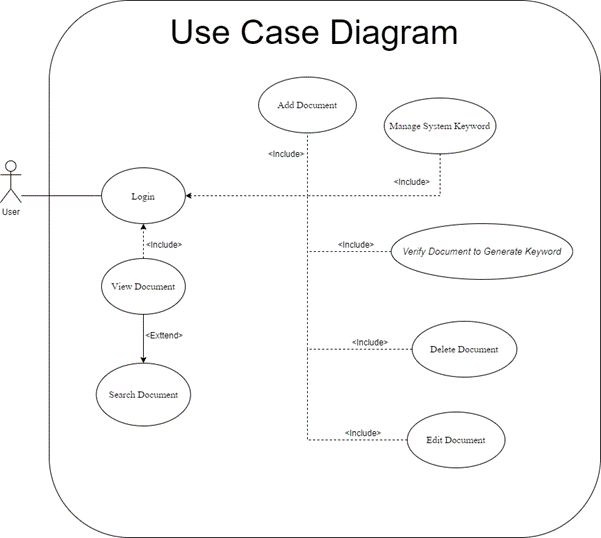
\includegraphics{usecasediagram}
    \caption{Use case diagram}\label{fig:usecasediagram}
\end{figure}

\subsection{Sequence diagram}

\subsubsection{Use case Add Document}

Scenario 1: เพิ่มหนังสือ/เอกสารเข้าสู่ระบบ

Goal: เพิ่มข้อมูลของเอกสารเข้าไปอยู่ในระบบ

Precondition: กดไปที่หัวข้อ INSERT BOOK ใน Web Application 

Main success scenario:

\begin{enumerate}
    \item อัพโหลดเอกสาร/หนังสือเลือกหน้าที่จะให้เริ่มต้นการแปลง
    \item กรอกข้อมูลรายละเอียดที่ต้องการลงในระบบ
    \item แสดงสถานะของการเพิ่มข้อมูล
    \item เพิ่มเอกสาร/หนังสือเข้าสู่ระบบ
\end{enumerate}

\begin{figure}[H]
    \centering
    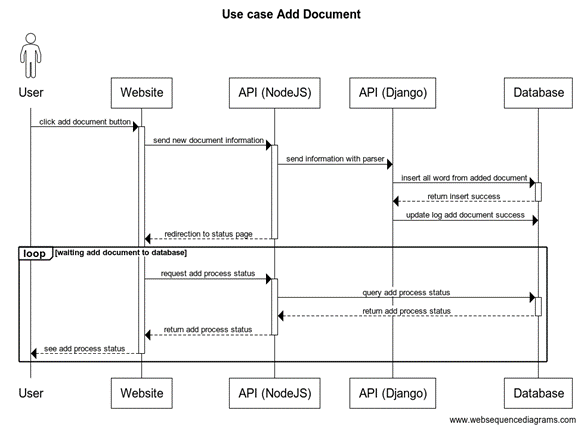
\includegraphics{scene1}
    \caption{แสดง Scenario 1 เพิ่มเอกสารเข้าระบบ}\label{fig:scene1}
\end{figure}

\subsubsection{Use case Manage word in document}

Scenario 2: การตรวจสอบและแก้ไขคำก่อนนำเข้าสู่ระบบ

Goal: ผู้ใช้งานเห็นคำที่จะถูกการแปลงเป็นดิจิตอลแล้วสามารถจัดการคำเหล่านั้นได้

Precondition: อยู่ภายในขั้นตอนการเพิ่มหนังสือ/เอกสารลงในระบบ

Main success scenario:

\begin{enumerate}
    \item ผู้ใช้เข้าไปยังหน้าดูสถานะการเพิ่มเอกสาร
    \item ผู้ใช้เลือกเอกสารที่อยู่ในสถานะตรวจสอบคำ
    \item ระบบแสดงคำทั้งหมดที่ถูกแปลงมาได้จากเอกสารแต่ละหน้า
    \item ผู้ใช้ตรวจสอบ แก้ไขคำที่แสดงขึ้นมา
    \item ยืนยันขั้นตอนการตรวจสอบและแก้ไขคำ
\end{enumerate}
\begin{figure}[H]
    \centering
    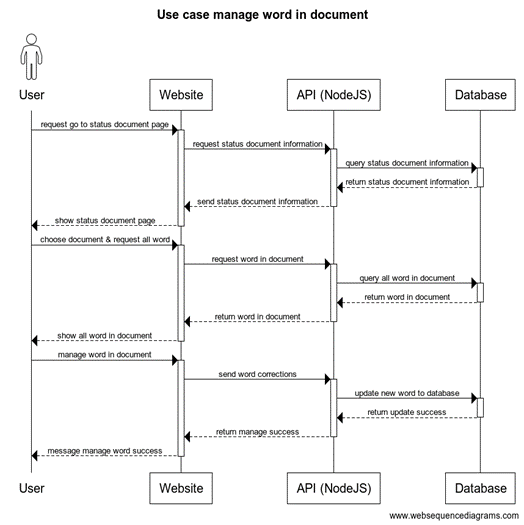
\includegraphics{scene2}
    \caption{แสดง Scenario 2 การจัดการคำที่ถูกเก็บได้จากเอกสารในระบบ}\label{fig:scene2}
\end{figure}

\subsubsection{Use case Verify Document to Generate Keyword}

Scenario 3: ยื่นเอกสารว่าพร้อมสำหรับการถูกนำไปสร้างคียเวิร์ด

Goal: เอกสารถูกยืนยันพร้อมกับสร้างคีย์เวิร์ดเพื่อเพิ่มเข้าไปในระบบ

Precondition: ไปยังหน้าสถานะของเอกสารแล้วกดไปยังปุ่มยืนยันเอกสารถูกต้อง

Main success scenario:

\begin{enumerate}
    \item ผู้ใช้เข้าไปยังหน้าดูสถานะการเพิ่มเอกสาร
    \item ระบบแสดงสถานะเอกสารว่าเอกสารไหนอยู่สถานะใดแล้วบ้าง
    \item ผู้ใช้กดยืนยันว่าเอกสารถูกต้อง
    \item ระบบย้ายไปหน้าสถานะเอกสารอีกครั้งเพื่อรอผลการทำงาน
    \item ระบบแสดงการยืนยันเอกสาร และถูกเพื่อคีย์เวิร์ดเสร็จสิ้น
\end{enumerate}
\begin{figure}[H]
    \centering
    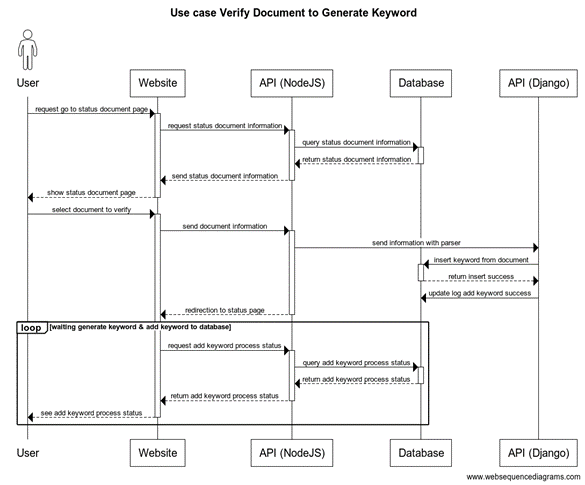
\includegraphics{scene3}
    \caption{แสดง Scenario 3 ยืนเอกสารว่าพร้อมสำหรับการถูกนำไปสร้างคีย์เวิร์ด}\label{fig:scene3}
\end{figure}

\subsubsection{Use case Edit Document}

Scenario 4: การแก้ไขรายละเอียดของเอกสาร/หนังสือที่อยู่ภายในระบบ

Goal: รายละเอียดเอกสารถูกแก้ไขตามผู้ใช้งานต้องการ

Precondition: กดไปที่หัวข้อ MANAGE BOOK ใน Web Application

Main success scenario:

\begin{enumerate}
    \item ผู้ใช้ค้นหาเอกสารที่ต้องการแก้ไขรายละเอียด
    \item แสดงผลลัพธ์ในการค้นหาเอกสาร/หนังสือ
    \item เลือกเอกสาร/หนังสือที่ต้องการแก้ไขรายละเอียด
    \item แก้ไขรายละเอียดที่ต้องการ
    \item กดบันทึกข้อมูลลงไปในระบบ
\end{enumerate}
\begin{figure}[H]
    \centering
    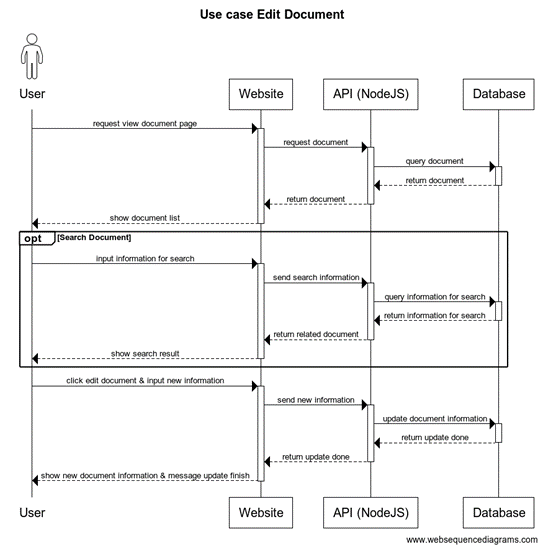
\includegraphics{scene4}
    \caption{แสดง Scenario 4 แก้ไขข้อมูลเอกสาร}\label{fig:scene4}
\end{figure}

\subsubsection{Use case Delete Document}

Scenario 5: ลบเอกสาร/หนังสือภายในระบบ

Goal: เอกสาร/หนังสือถูกนำออกจากระบบ

Precondition: กดเลือกหัวข้อ MANAGE BOOK ใน Web Application

Main success scenario:

\begin{enumerate}
    \item ผู้ใช้ทำการค้นหาเอกสารหนังสือที่ต้องการจะลบออกจากระบบ
    \item แสดงผลลัพธ์ในการค้นหาเอกสาร/หนังสือ
    \item กดลบเอกสาร/หนังสือที่ต้องการ
    \item กดยืนยันคำสั่งลบเพื่อบันทึกลงระบบ
\end{enumerate}
\begin{figure}[H]
    \centering
    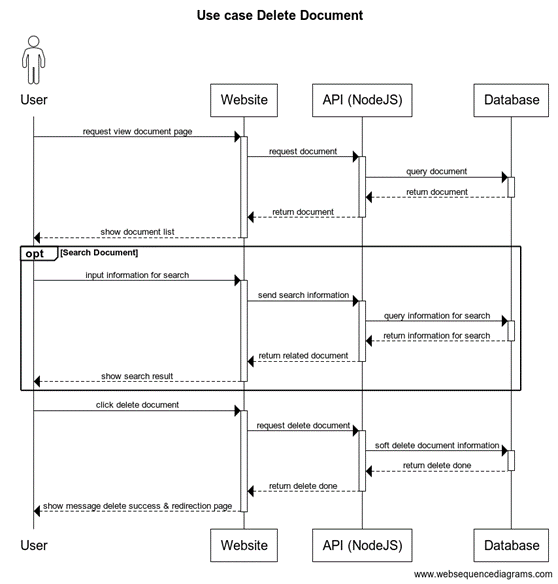
\includegraphics{scene5}
    \caption{แสดง Scenario 5 ลบเอกสาร}\label{fig:scene5}
\end{figure}

\subsubsection{Use case View Document \& Search Document}

Scenario 6: ดูข้อมูลเอกสาร และการค้นหาเอกสาร

Goal: ผู้ใช้เจอเอกสารที่ต้องการ

Precondition: กดไปที่หัวข้อ SEARCH ใน Web Application

Main success scenario:

\begin{enumerate}
    \item กรอกรายละเอียดข้อมูลที่ต้องการจะค้นหา
    \item แสดงผลลัพธ์ในการค้นหา
    \item ผู้ใช้เลือกเอกสารที่ต้องการที่จะดูข้อมูล
    \item ระบบย้ายไปยังหน้าแสดงข้อมูลเอกสารที่ถูกเลือก
\end{enumerate}
\begin{figure}[H]
    \centering
    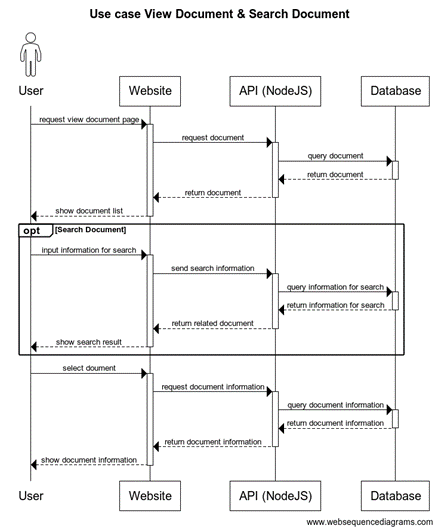
\includegraphics{scene6}
    \caption{แสดง Scenario 6 ดูข้อมูลเอกสาร และการค้นหาเอกสาร}\label{fig:scene6}
\end{figure}

\subsubsection{Use case Login}

Scenario 7: ระบบล็อกอิน

Goal: เพื่อเข้าสู่ระบบให้สามารถใช้ฟังก์ชั่นภายใน Web Application เพิ่มเติมได้

Precondition: กดหัวข้อ LOGIN ใน Web Application

Main success scenario:

\begin{enumerate}
    \item ผู้ใช้กรอกชื่อผู้ใช้งานและรหัสผ่าน
    \item กดเข้าสู่ระบบ
    \item เข้าสู่ระบบสำเร็จ ส่งผู้ใช้กลับไปสู่ Homepage
    \item สามารถเข้าใช้งานฟังก์ชั่นของ Web Application ได้
\end{enumerate}
\begin{figure}[H]
    \centering
    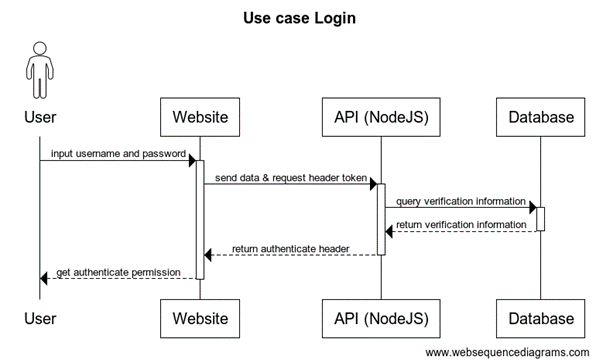
\includegraphics{scene7}
    \caption{แสดง Scenario 7 ระบบล็อกอิน}\label{fig:scene7}
\end{figure}

\section{GUI Design}

\subsection{Homepage}
\begin{figure}[H]
    \centering
    
\includegraphics[scale=0.3]{hp}
    \caption{ภาพแสดงหน้าหลักของเว็บไซต์}\label{fig:hp}
\end{figure}
หน้าหลักของเว็บไซต์จะเป็นหน้าที่เน้นการค้นหาเป็นหลัก ที่ผู้ใช้สามารถเข้าถึงเมนูการเพิ่มหนังสือ การจัดการ และการเข้าสู่ระบบได้ที่แถบ Navigation ด้านบนของเว็บไซต์ดังรูปที่ \ref{fig:hp}

\subsection{Homepage2}
\begin{figure}[H]
    \centering
    
\includegraphics[scale=0.3]{hp2}
    \caption{ภาพแสดงหน้าหลักของเว็บไซต์หลังจากการกดเปิดเมนู}\label{fig:hp2}
\end{figure}
เมื่อกดปุ่มลูกศรที่ด้านล่างของรูป \ref{fig:hp} จะมีเมนูเพิ่มเติมขึ้นมากลายเป็นรูปที่ \ref{fig:hp2} ซึ่งจะแสดงรายละเอียดในแต่ละฟังก์ชั่นเพิ่มเติม

\subsection{Login}
\begin{figure}[H]
    \centering
    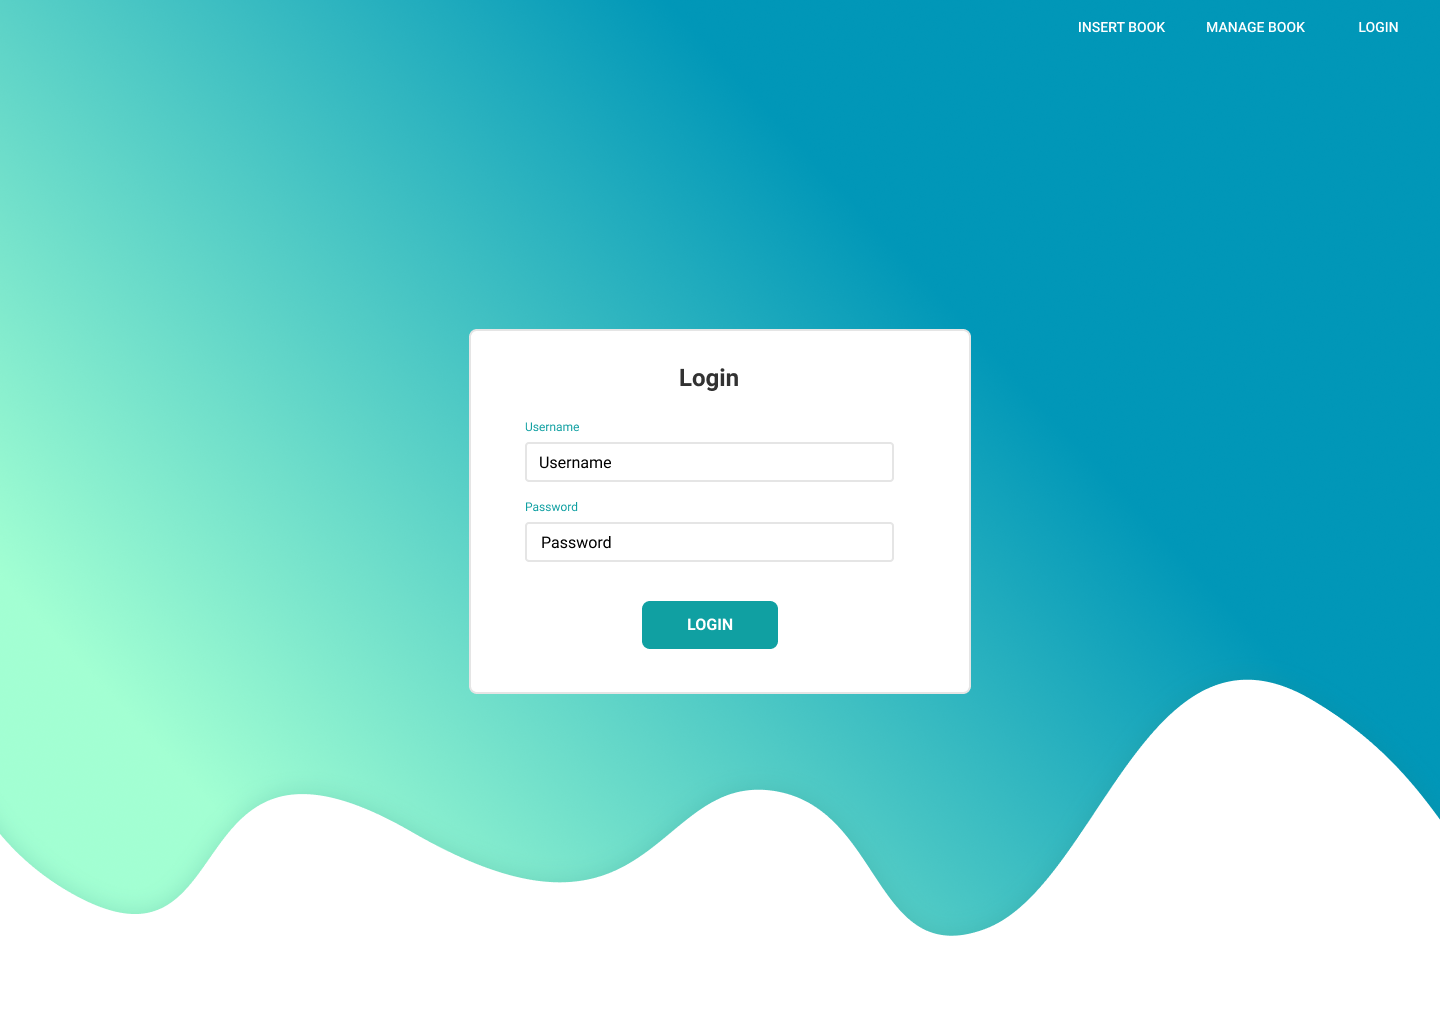
\includegraphics[scale=0.3]{login}
    \caption{ภาพแสดงหน้าเข้าสู่ระบบ}\label{fig:scene7}
\end{figure}
ก่อนที่จะทำการเพิ่มหนังสือหรือจัดการกับหนังสือผู้ใช้นั้นจะต้องเข้าสู่ระบบก่อนเสมอ ถ้าเกิดกดเข้าฟังก์ชั่นการเพิ่มหนังสือหรือค้นหาโดยที่ยังไม่ได้เข้าสู่ระบบ ระบบจะบังคับให้ผู้ใช้เข้ามาในหน้าเข้าสู่ระบบดังรูป 3.25 เพื่อทำการเข้าสู่ระบบหรือจะเข้ามาโดยการกด log in ที่ปุ่มขวาบนได้

\subsection{Insert Book(1)}
\begin{figure}[H]
    \centering
    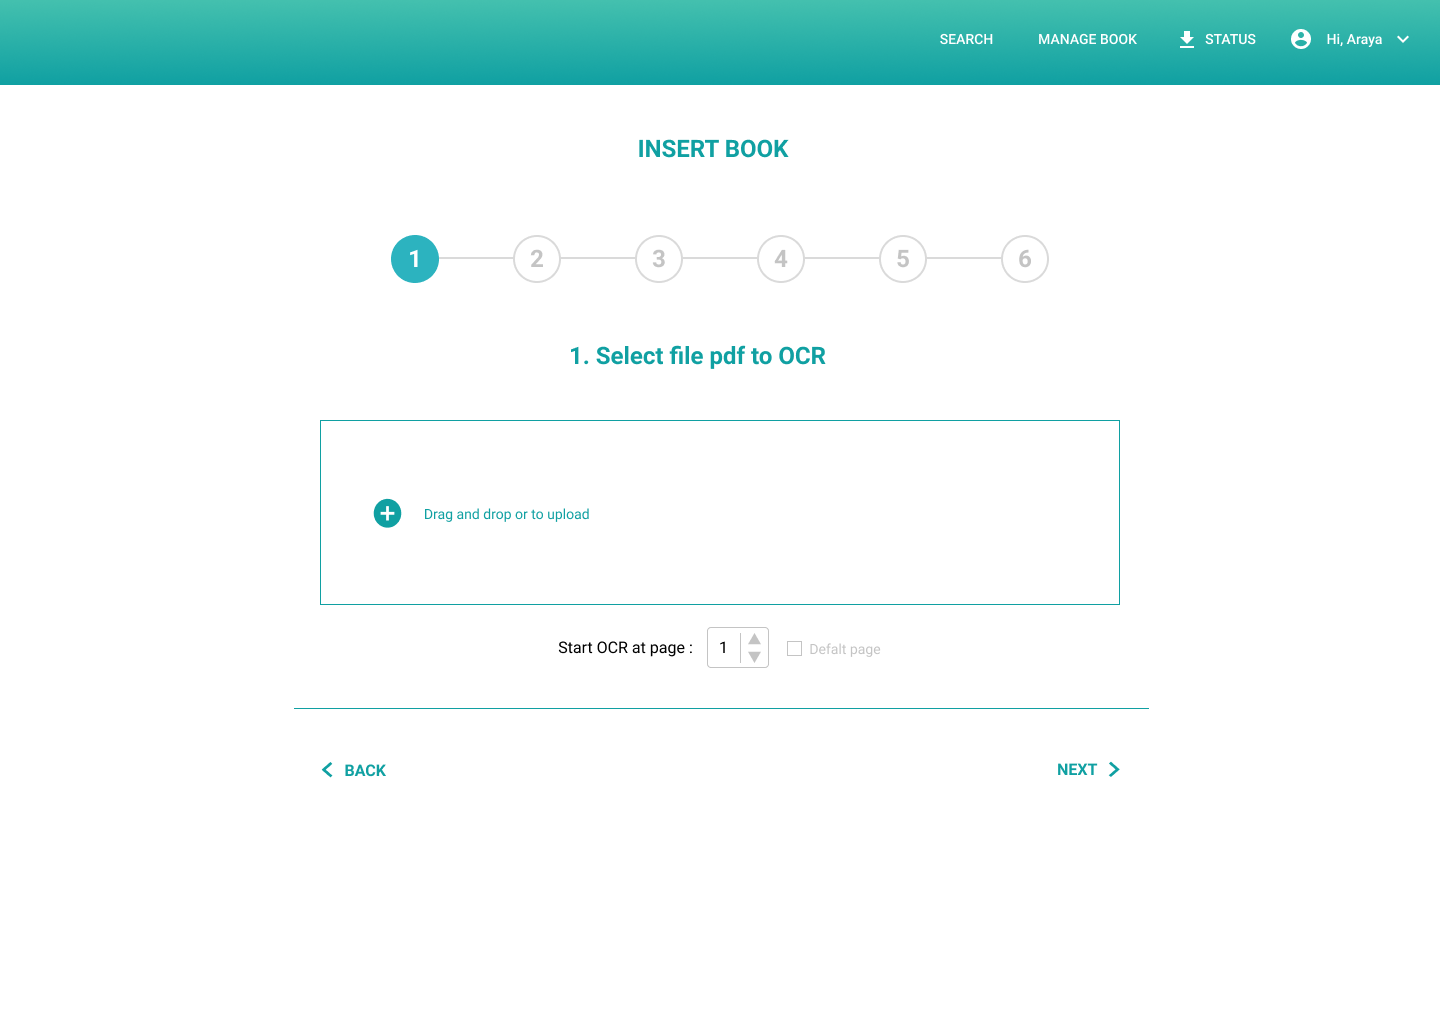
\includegraphics[scale=0.27]{i1}
    \caption{ภาพแสดงขั้นตอนการเพิ่มหนังสือเข้าสู่ระบบขั้นเลือกไฟล์}\label{fig:i1}
\end{figure}
หน้าเพิ่มหนังสือขั้นแรกจะเป็นการเลือกไฟล์เอกสารที่ต้องการโดยที่จะมีส่วนของการเพิ่มไฟล์ที่อยู่รูปของ pdf เพื่อทำ OCR จากนั้นจะสามารถเลือกได้ว่าจะทำการ OCR ตั้งแต่หน้าไหนดังรูปที่ 3.26

\subsection{Insert Book (2) }
\begin{figure}[H]
    \centering
    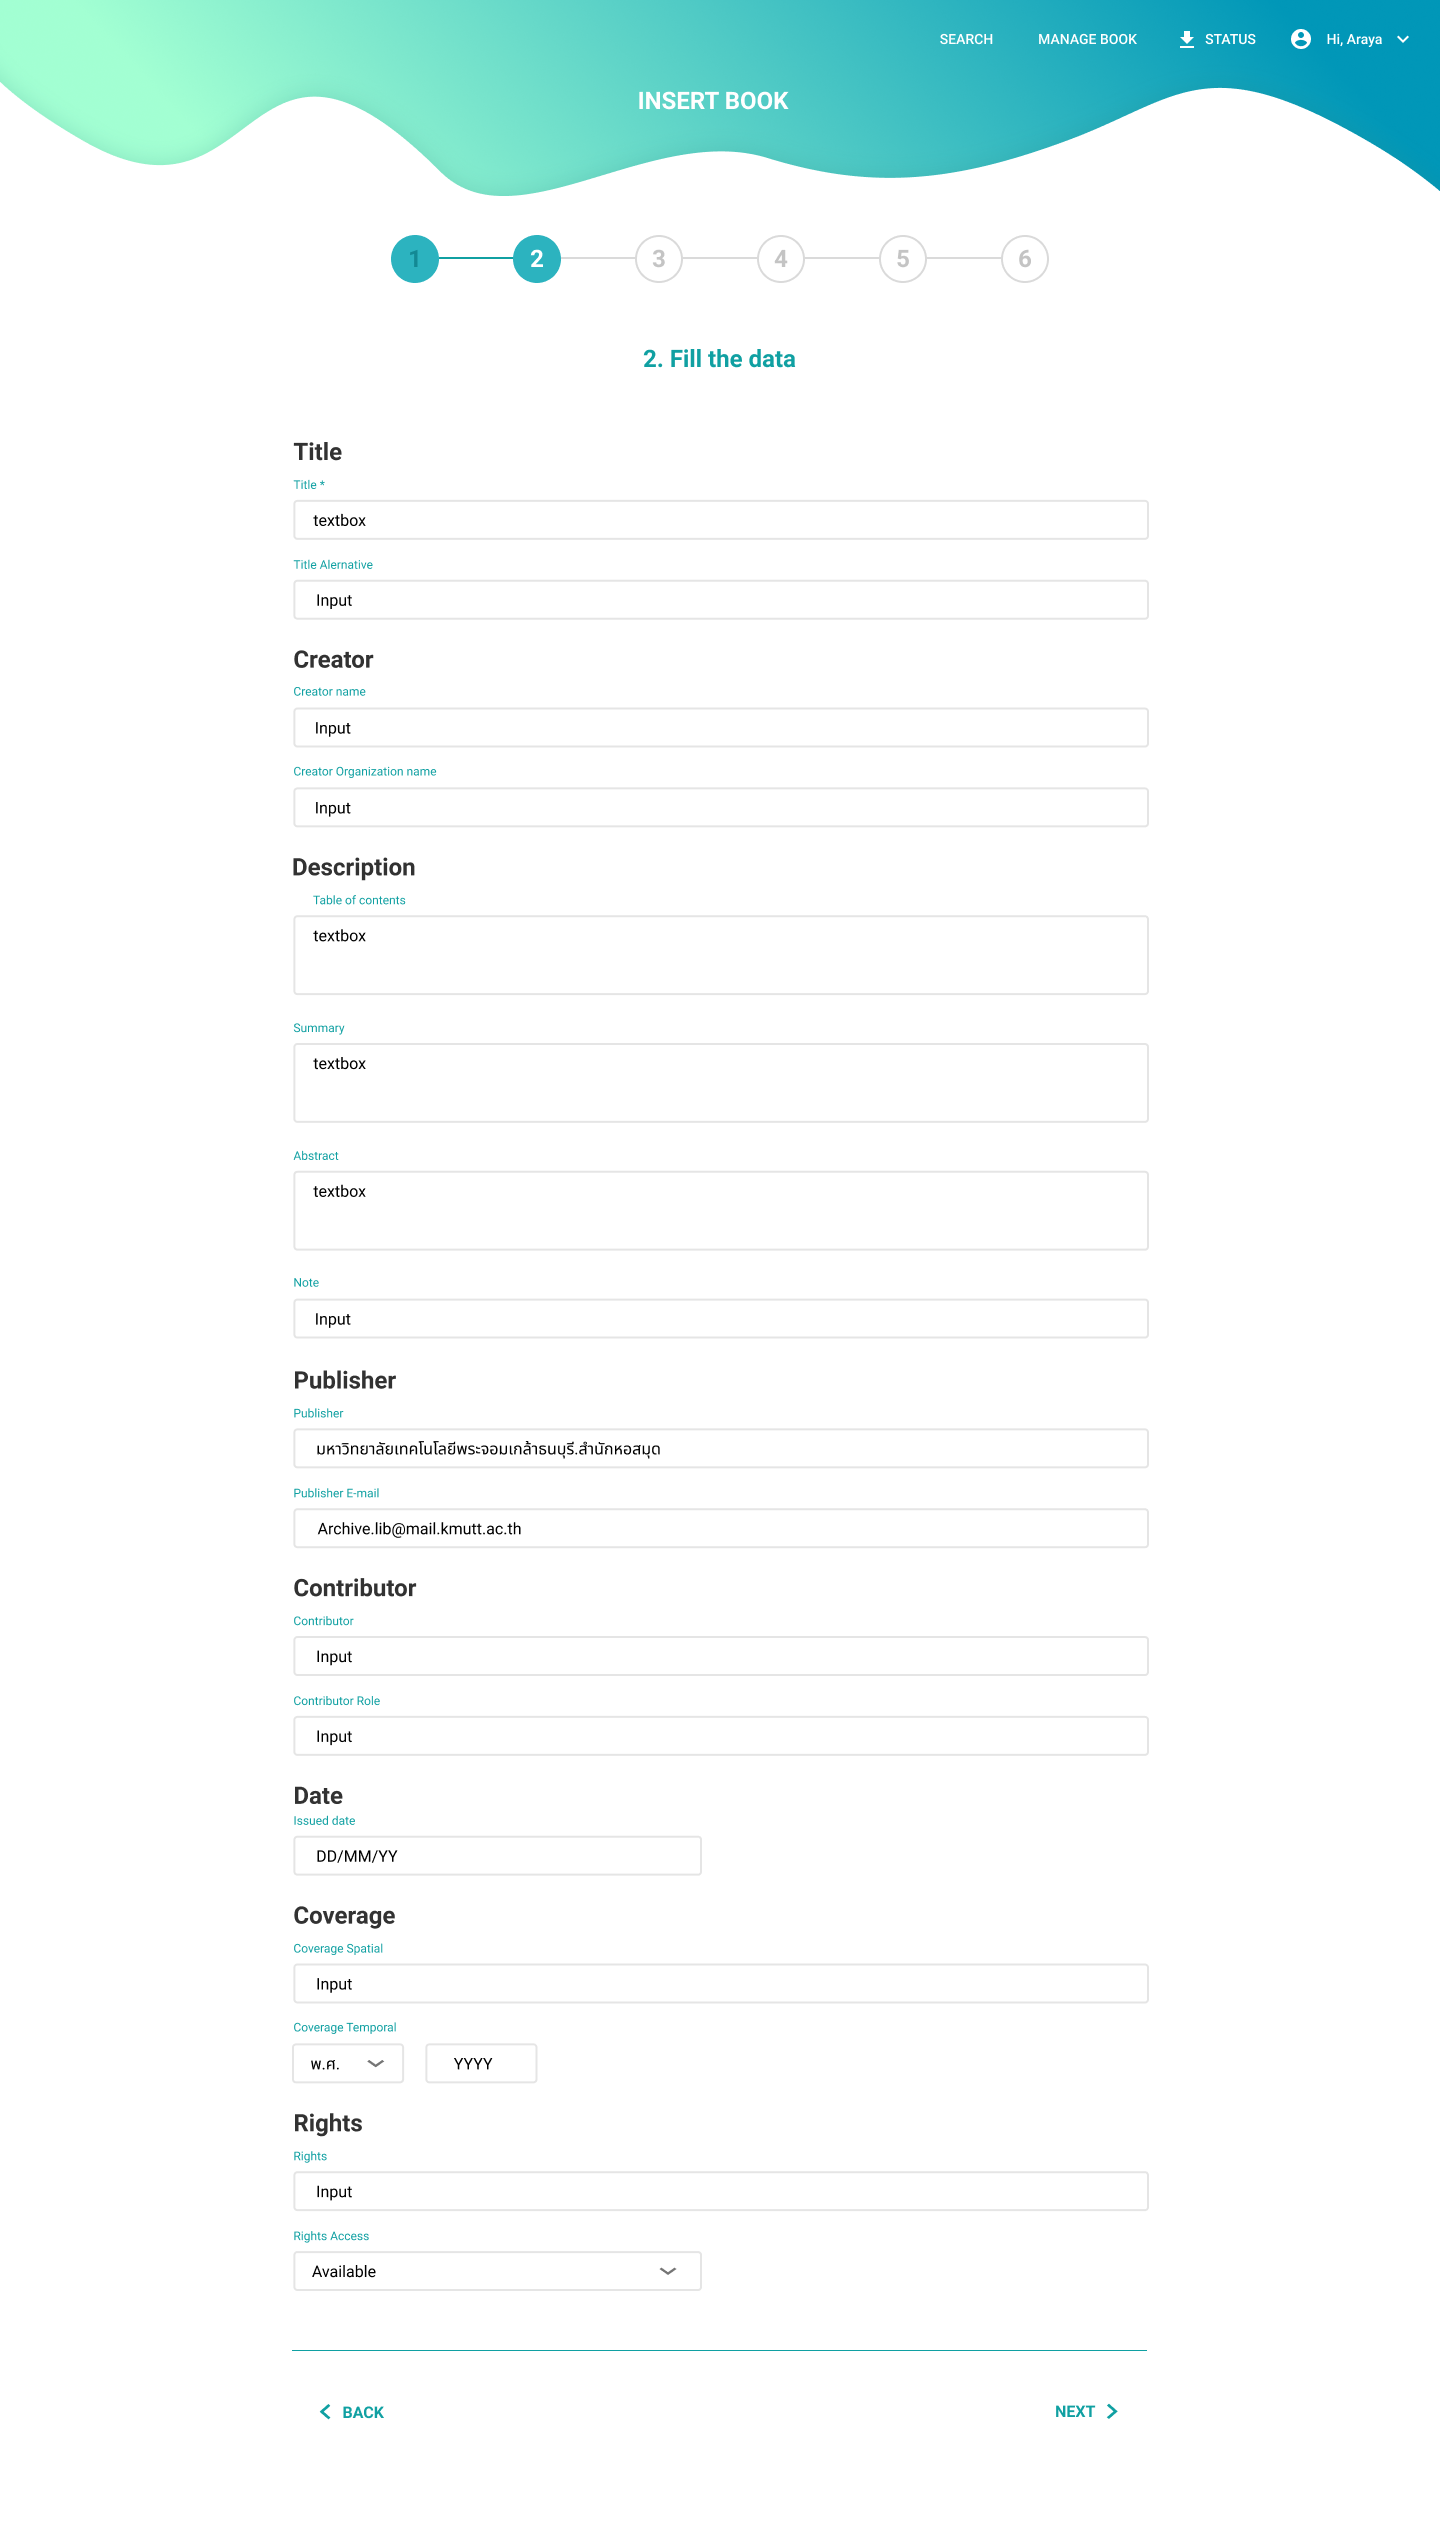
\includegraphics[scale=0.3]{i2}
    \caption{ภาพแสดงขั้นตอนการเพิ่มหนังสือเข้าสู่ระบบขั้นกรอกข้อมูลขั้นที่ 1}\label{fig:i2}
\end{figure}
หน้าเพิ่มหนังสือขั้นตอนที่ 2 เป็นหน้าที่ต้องใส่ข้อมูลที่จำเป็นของหนังสือ โดยที่จำเป็นต้องใส่จะมีสัญลักษณ์กำกับไว้หรือก็คือชื่อหนังสือดังรูป 3.27 โดยในหน้านี้จะมีกล่องใส่ข้อมูลที่ถูกกรอกบ่อย ๆสำหรับผู้ใช้(เจ้าหน้าที่)

\subsection{Insert Book (3)}
\begin{figure}[H]
    \centering
    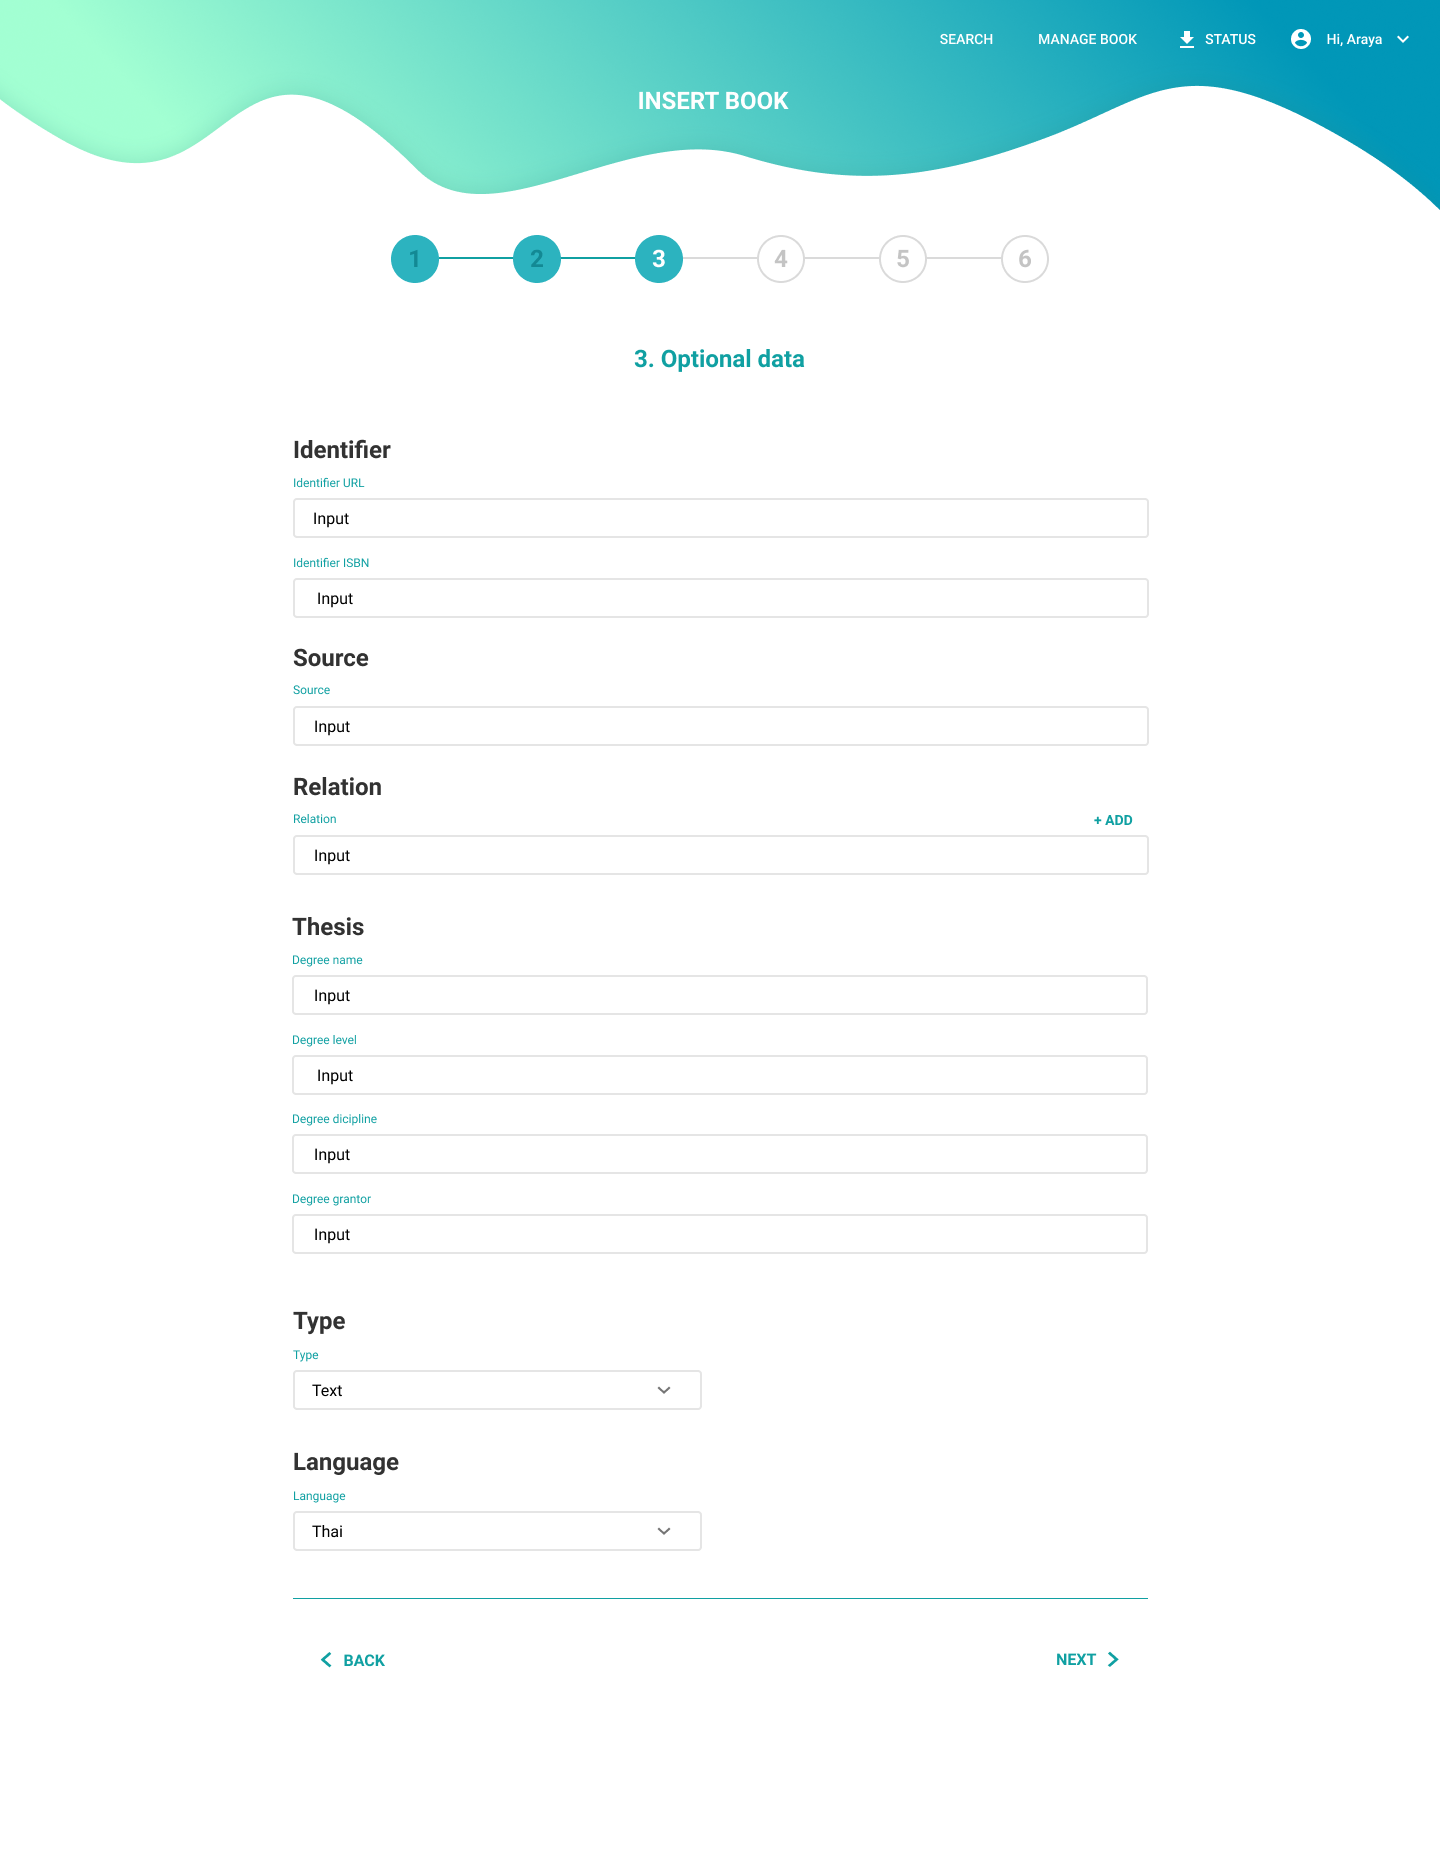
\includegraphics[scale=0.3]{i3}
    \caption{ภาพแสดงขั้นตอนการเพิ่มหนังสือเข้าสู่ระบบขั้นกรอกข้อมูลขั้นที่ 2}\label{fig:i3}
\end{figure}
ในขั้นตอนที่ 3 จากรูปที่ 3.28 จะเป็นหน้าที่ใส่ข้อมูลที่ส่วนใหญ่ผู้ใช้จะไม่ค่อยกรอกมากนัก ซึ่งไม่มีกล่องข้อมูลไหนจำเป็นที่ต้องกรอกผู้ใช้สามารถข้ามไปขั้นตอนถัดไปได้เลย

\subsection{Insert Book (4)}
\begin{figure}[H]
    \centering
    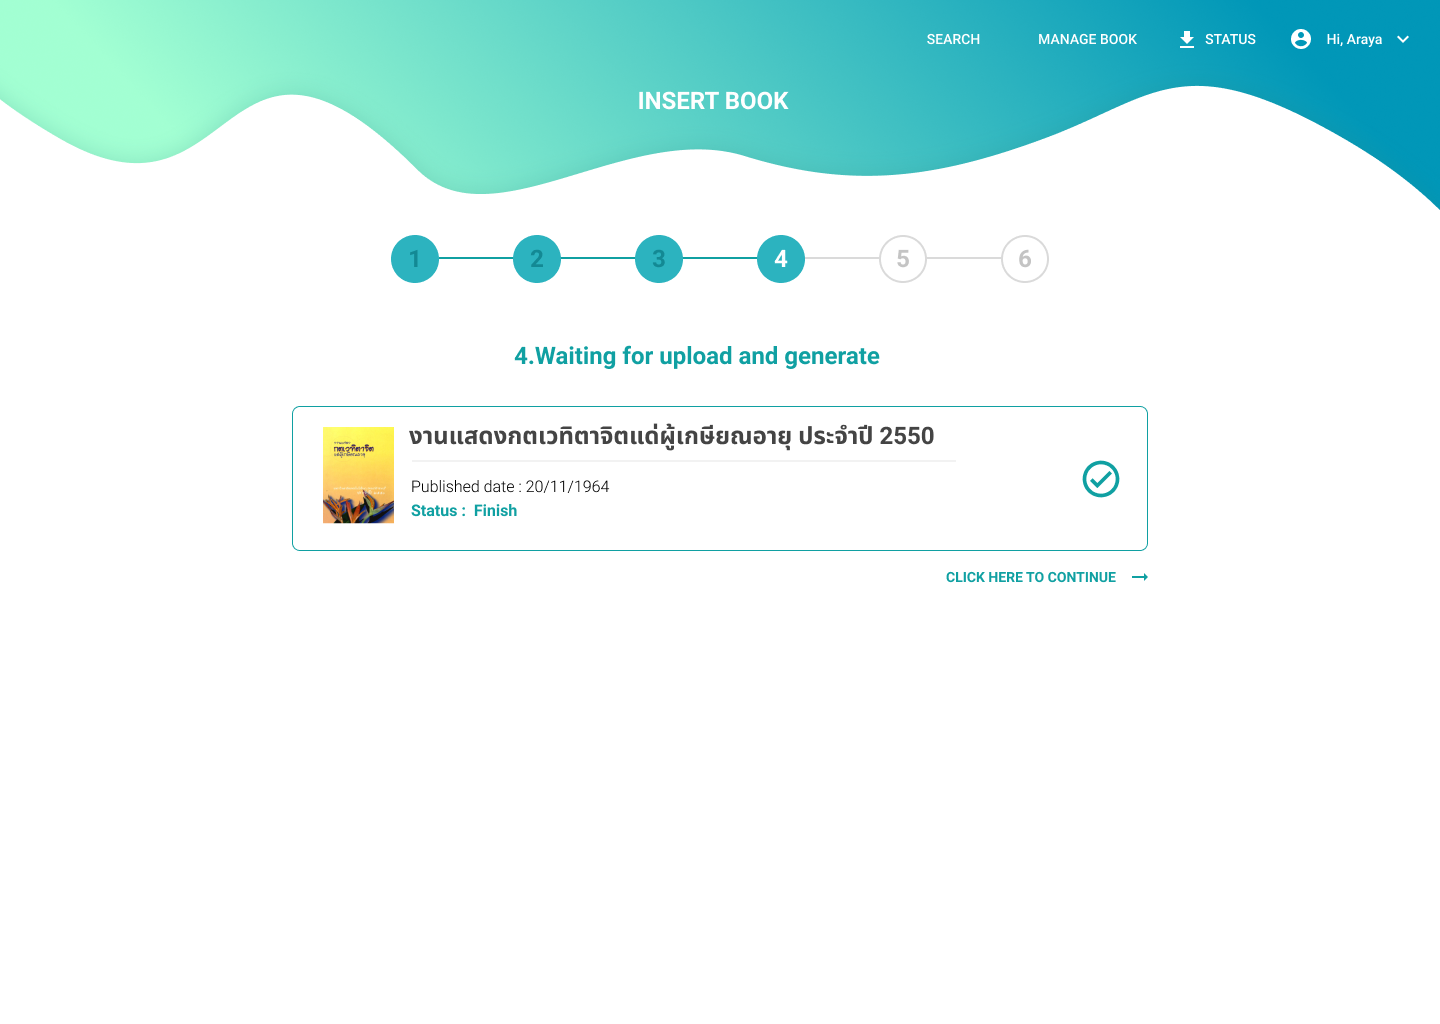
\includegraphics[scale=0.3]{i4}
    \caption{ภาพแสดงขั้นตอนการเพิ่มหนังสือเข้าขั้นโหลดข้อมูลเข้าสู่ระบบ}\label{fig:i4}
\end{figure}
หลังจากที่ทำการใส่ข้อมูลออกมาทั้งหมดแล้วมาถึงหน้าที่เป็นหน้าโหลดข้อมูลดังรูป 3.29 ที่ระบบจะทำการ OCR และทำการเตรียมชุดข้อมูลที่ได้จากการ OCR โดยการนำคำมาตัดและเช็คคำผิด เมื่อโหลดข้อมูลเสร็จแล้วระบบจะทำการเปลี่ยนสถานะการโหลดและขึ้นลิ้งเพื่อเข้าสู่ขั้นตอนถัดไปได้

\subsection{Insert Book (5)}
\begin{figure}[H]
    \centering
    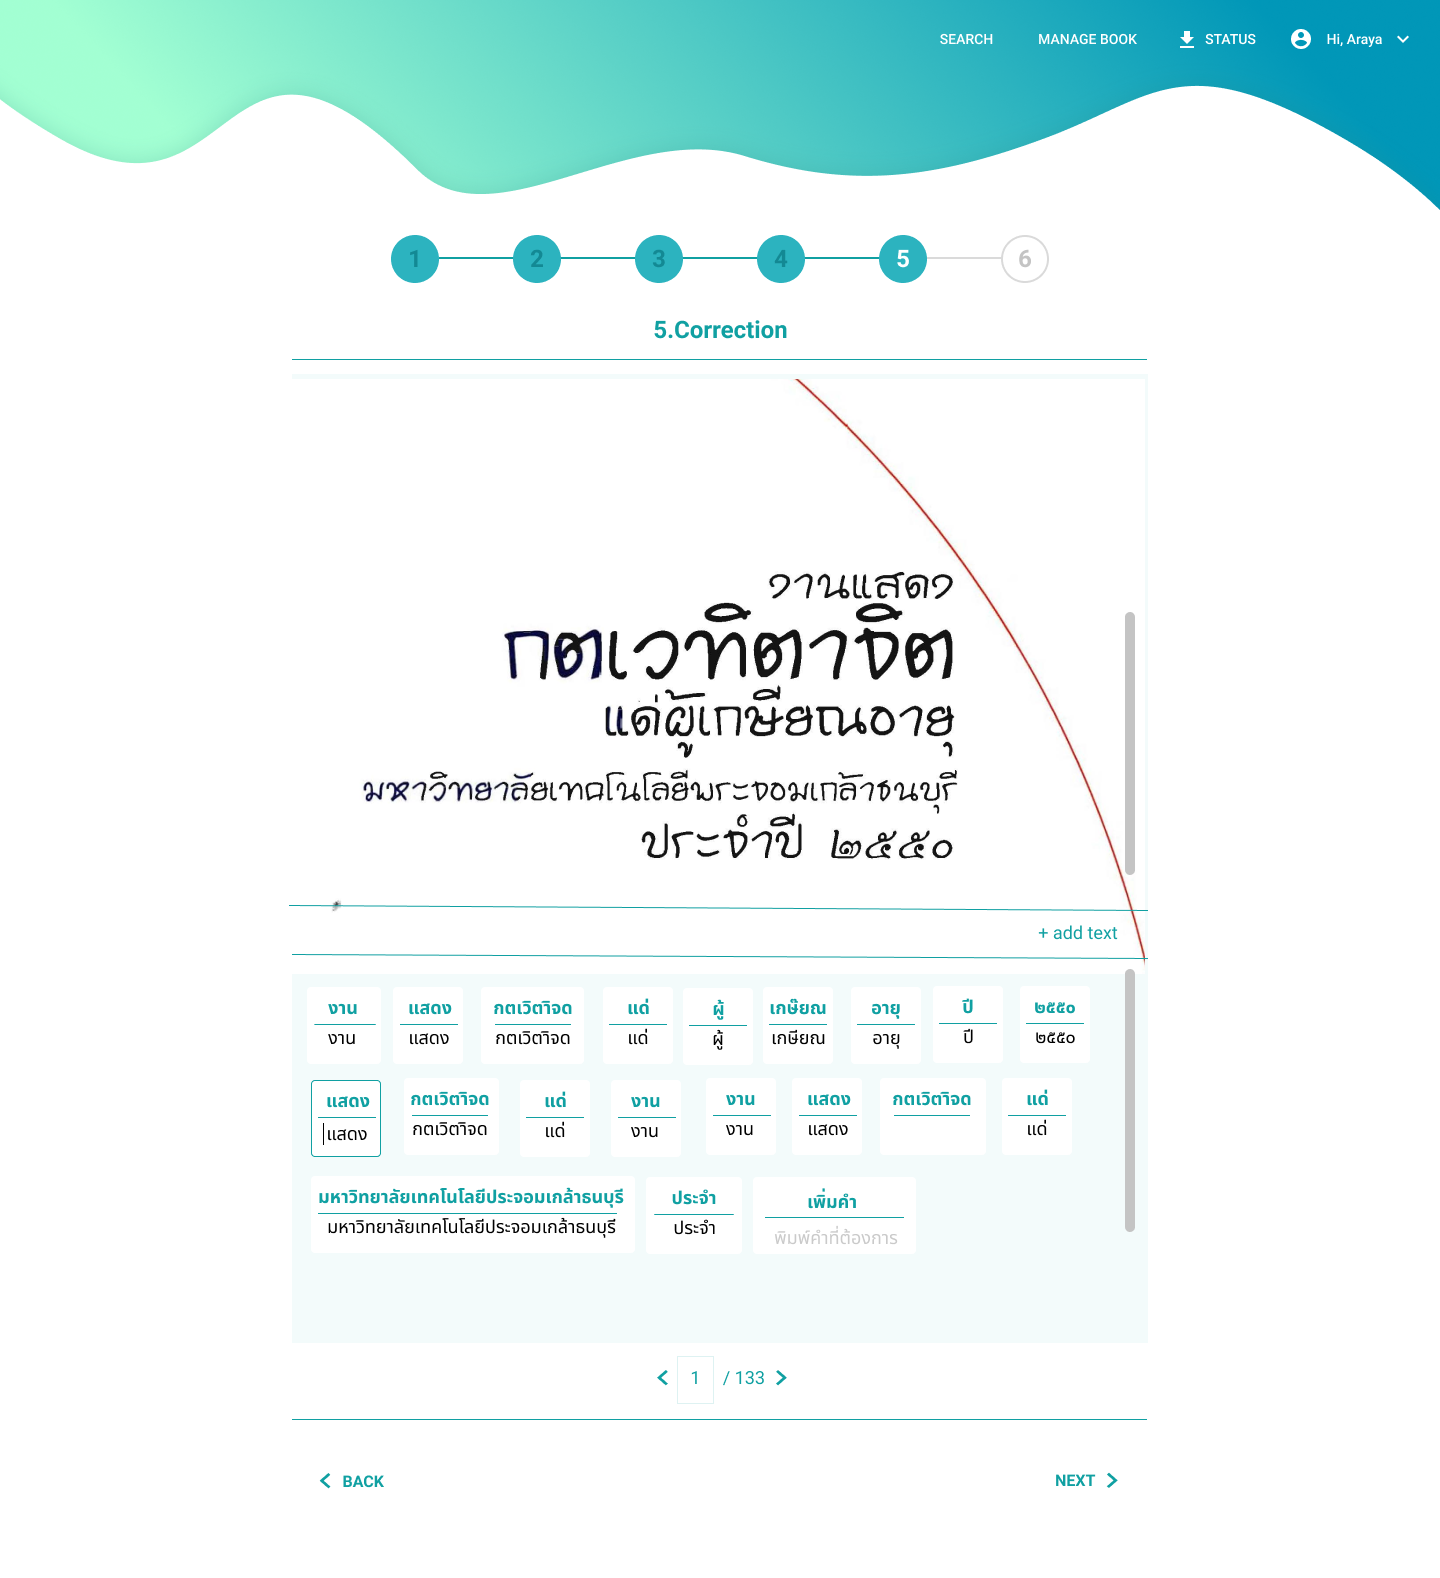
\includegraphics[scale=0.3]{i5}
    \caption{ภาพแสดงขั้นตอนการเพิ่มหนังสือเข้าสู่ระบบขั้นแก้ไขคำผิด}\label{fig:i5}
\end{figure}
หลังจากโหลดและเตรียมข้อมูลเรียบร้อยแล้ว ระบบจะทำการแสดงข้อมูลที่ถูกแปลงมาโดยที่ผู้ใช้จะสามารถแก้ไขคำได้ดังรูป 3.30 หรือสามารถข้ามได้เลยเช่นกัน โดยเมื่อคลิกไปที่กล่องข้อความจะขึ้นให้แก้แต่ละคำและเมื่อเปลี่ยนหน้าจะทำการเก็บข้อมูลที่เปลี่ยนไว้ และจะบันทึกการแก้ไขข้อมูลทั้งหมดที่แก้เมื่อข้ามไปขั้นตอนถัดไป

\subsection{Insert Book (6) }
\begin{figure}[H]
    \centering
    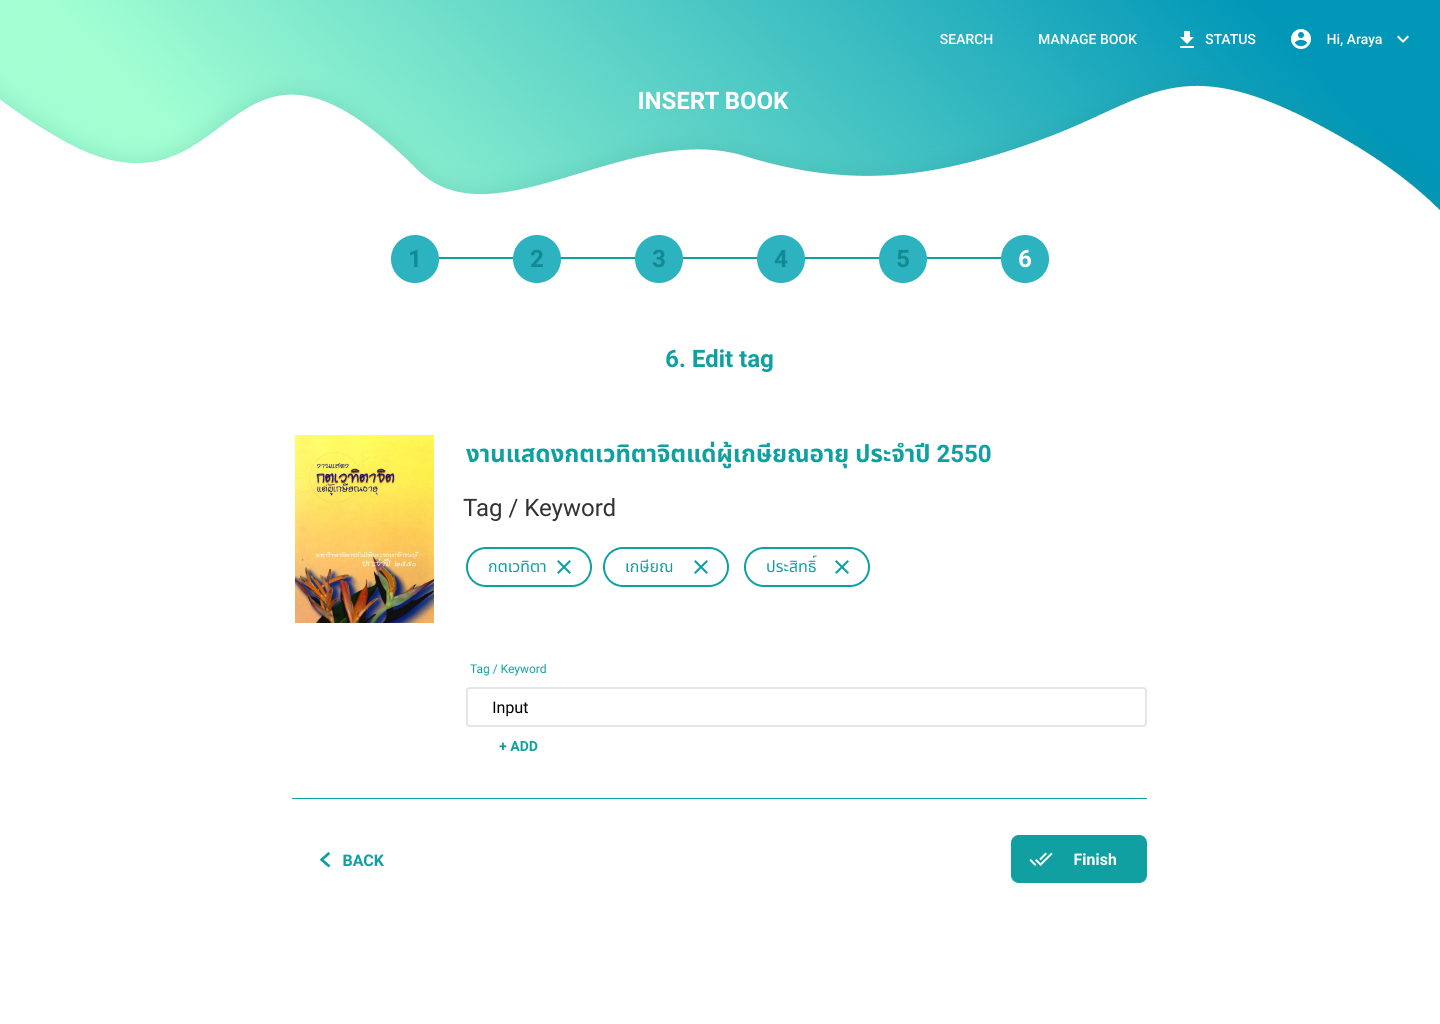
\includegraphics[scale=0.3]{i6}
    \caption{ภาพแสดงขั้นตอนการเพิ่มหนังสือเข้าสู่ระบบขั้นแก้ไขและเพิ่มคำสำคัญ}\label{fig:i6}
\end{figure}
หน้าสุดท้ายของการเพิ่มหนังสือจะเป็นหน้าที่ให้ผู้ใช้สามารถจัดการกับ Keyword ได้ดังรูปที่ 3.31 โดยเมื่อผู้ใช้ต้องการใส่คำสำคัญเพิ่มสามารถกด ADD เพื่อเพิ่มคำที่ต้องการใส่ได้ และสามารถลบเมื่อคลิกที่ปุ่มกากบาทที่คำสำคัญที่ระบบทำการสร้างมาให้ เมื่อแก้ไขเสร็จแล้วสามารถกดปุ่ม Finish เพื่อทำการบันทึกข้อมูล

\subsection{Search}
\begin{figure}[H]
    \centering
    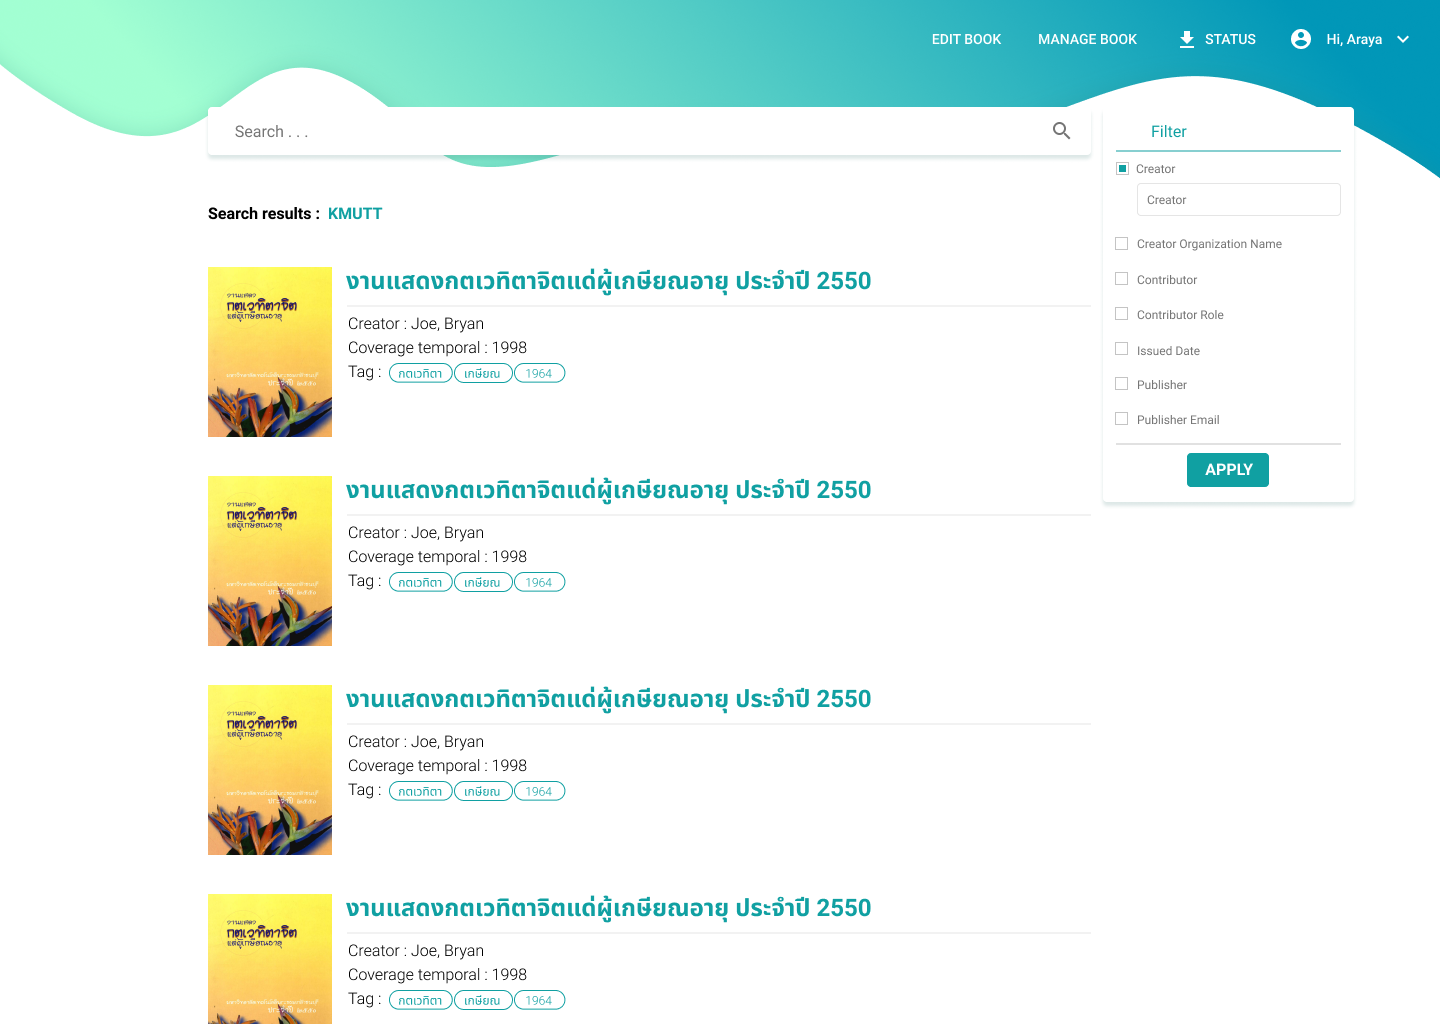
\includegraphics[scale=0.3]{search}
    \caption{ภาพแสดงหน้าค้นหาข้อมูล}\label{fig:search}
\end{figure}
หน้าแสดงข้อมูลการค้นหาเมื่อทำการค้นหาข้อมูลจากหน้าแรก (รูปที่ 3.23 หรือ 3.24) จะทำการแสดงข้อมูลหนังสือที่ตรงกับ keyword โดยเรียงคะแนนของหนังสือที่เกี่ยวข้องกับคำค้นหามากที่สุดดังรูปที่ 3.32 เมื่อกดเข้าไปที่รายชื่อหนังสือจะทำการนำทางผู้ใช้ไปยังหน้าดูหนังสือดังรูปที่ 3.33

\subsection{Document View}
\begin{figure}[H]
    \centering
    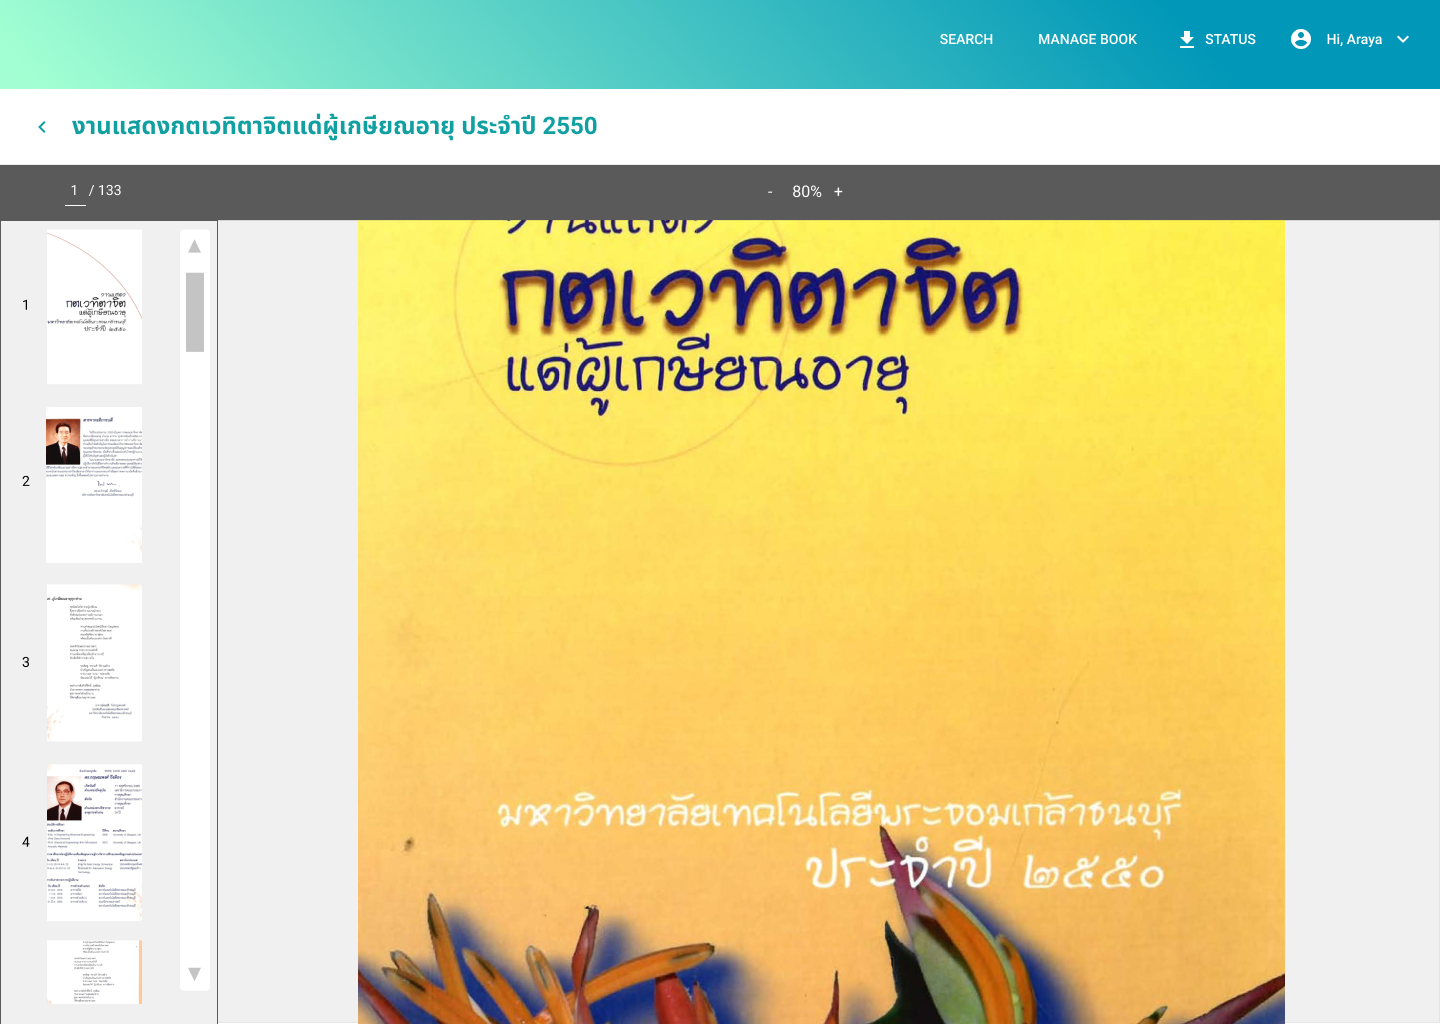
\includegraphics[scale=0.3]{lookupp}
    \caption{ภาพแสดงหน้าดูหนังสือ}\label{fig:lookupp}
\end{figure}
เมื่อเราค้นหาและเลือกหนังสือ ก็จะมีหน้าหนังสือ (รูปที่ 3.33) ขึ้นมาให้ดูเนื้อหาภายในโดยที่ผู้ใช้สามารถปรับขนาดภาพและสามารถเลือกหน้าที่ต้องการจะเปิดได้และสามารถย้อนหลับไปยังหน้าเสริชได้ที่ปุ่มลูกศรทางด้านซ้ายบน

\subsection{Manage book}
\begin{figure}[H]
    \centering
    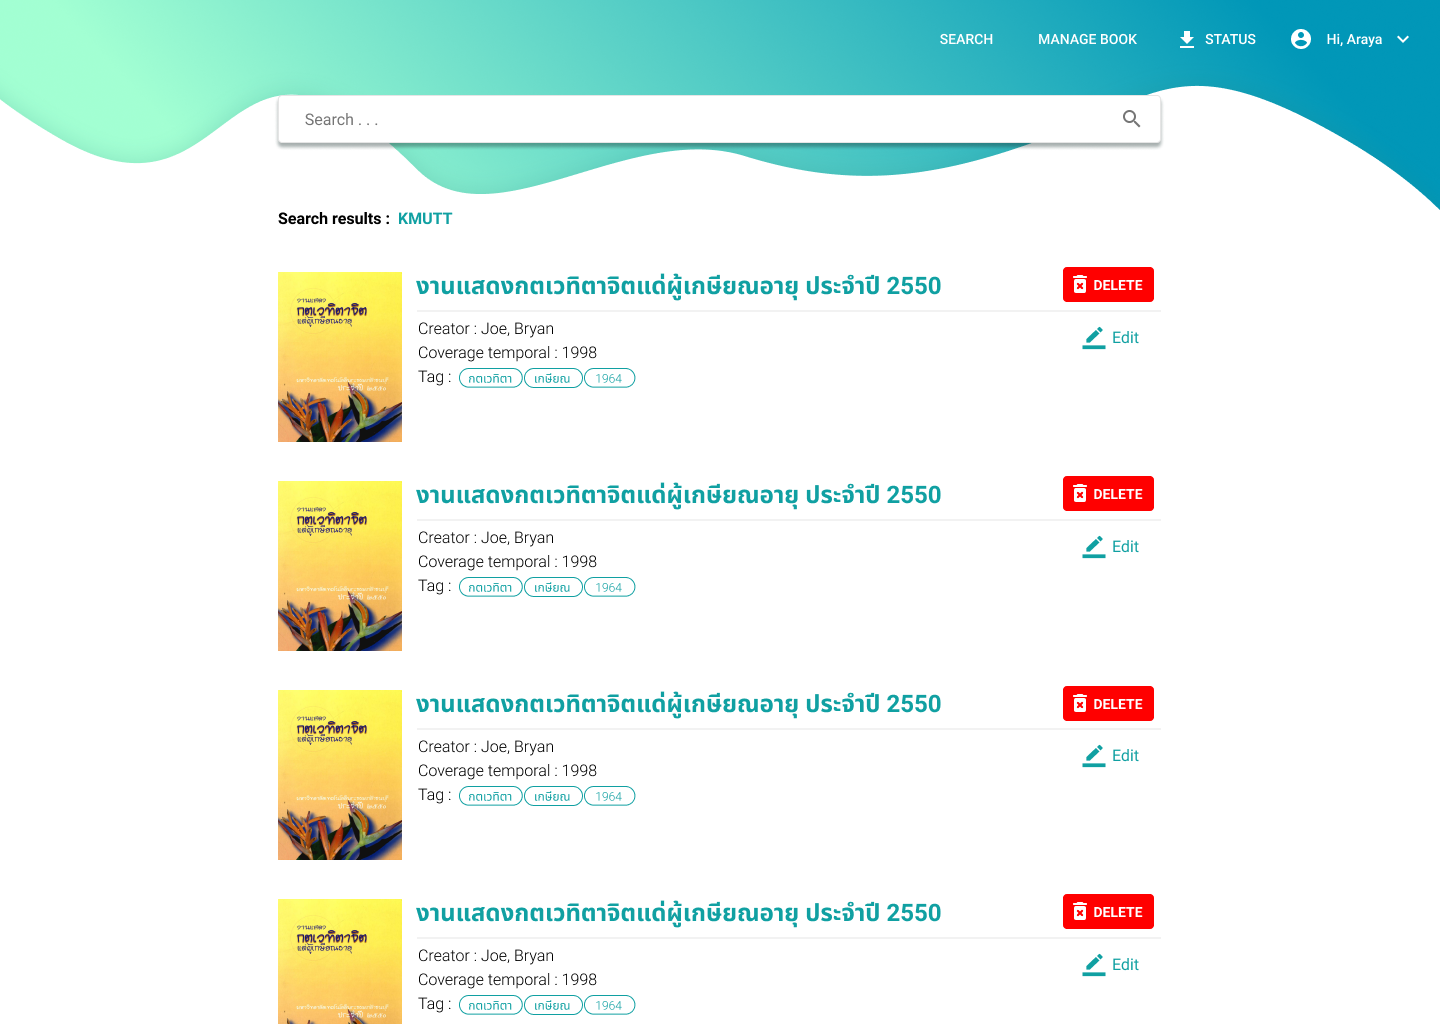
\includegraphics[scale=0.3]{man1}
    \caption{ภาพแสดงหน้าการจัดการหนังสือที่เพิ่มเข้าสู่ระบบ}\label{fig:man1}
\end{figure}
ในหน้าของการจัดการหนังสือดังรูปที่ 3.34 จะมีลักษณะคล้ายกับหน้าการค้นหาเพียงแต่ว่าจะมีฟังก์ชั่นสำหรับการแก้ไขเนื้อหนังสือภายในที่ผู้ใช้เคยกรอกไว้ตอน OCR หนังสือมา เมื่อกดปุ่มลบจะมีหน้าต่างแจ้งเตือนเพื่อถามความแน่ใจในการลบเอกสาร หรือกดปุ่ม Edit เพื่อทำการเข้าสู่การแก้ไขข้อมูลของเอกสารนั้นๆดังรูปที่ 3.35 - 3.37

\subsection{Edit Book}
\begin{figure}[H]
    \centering
    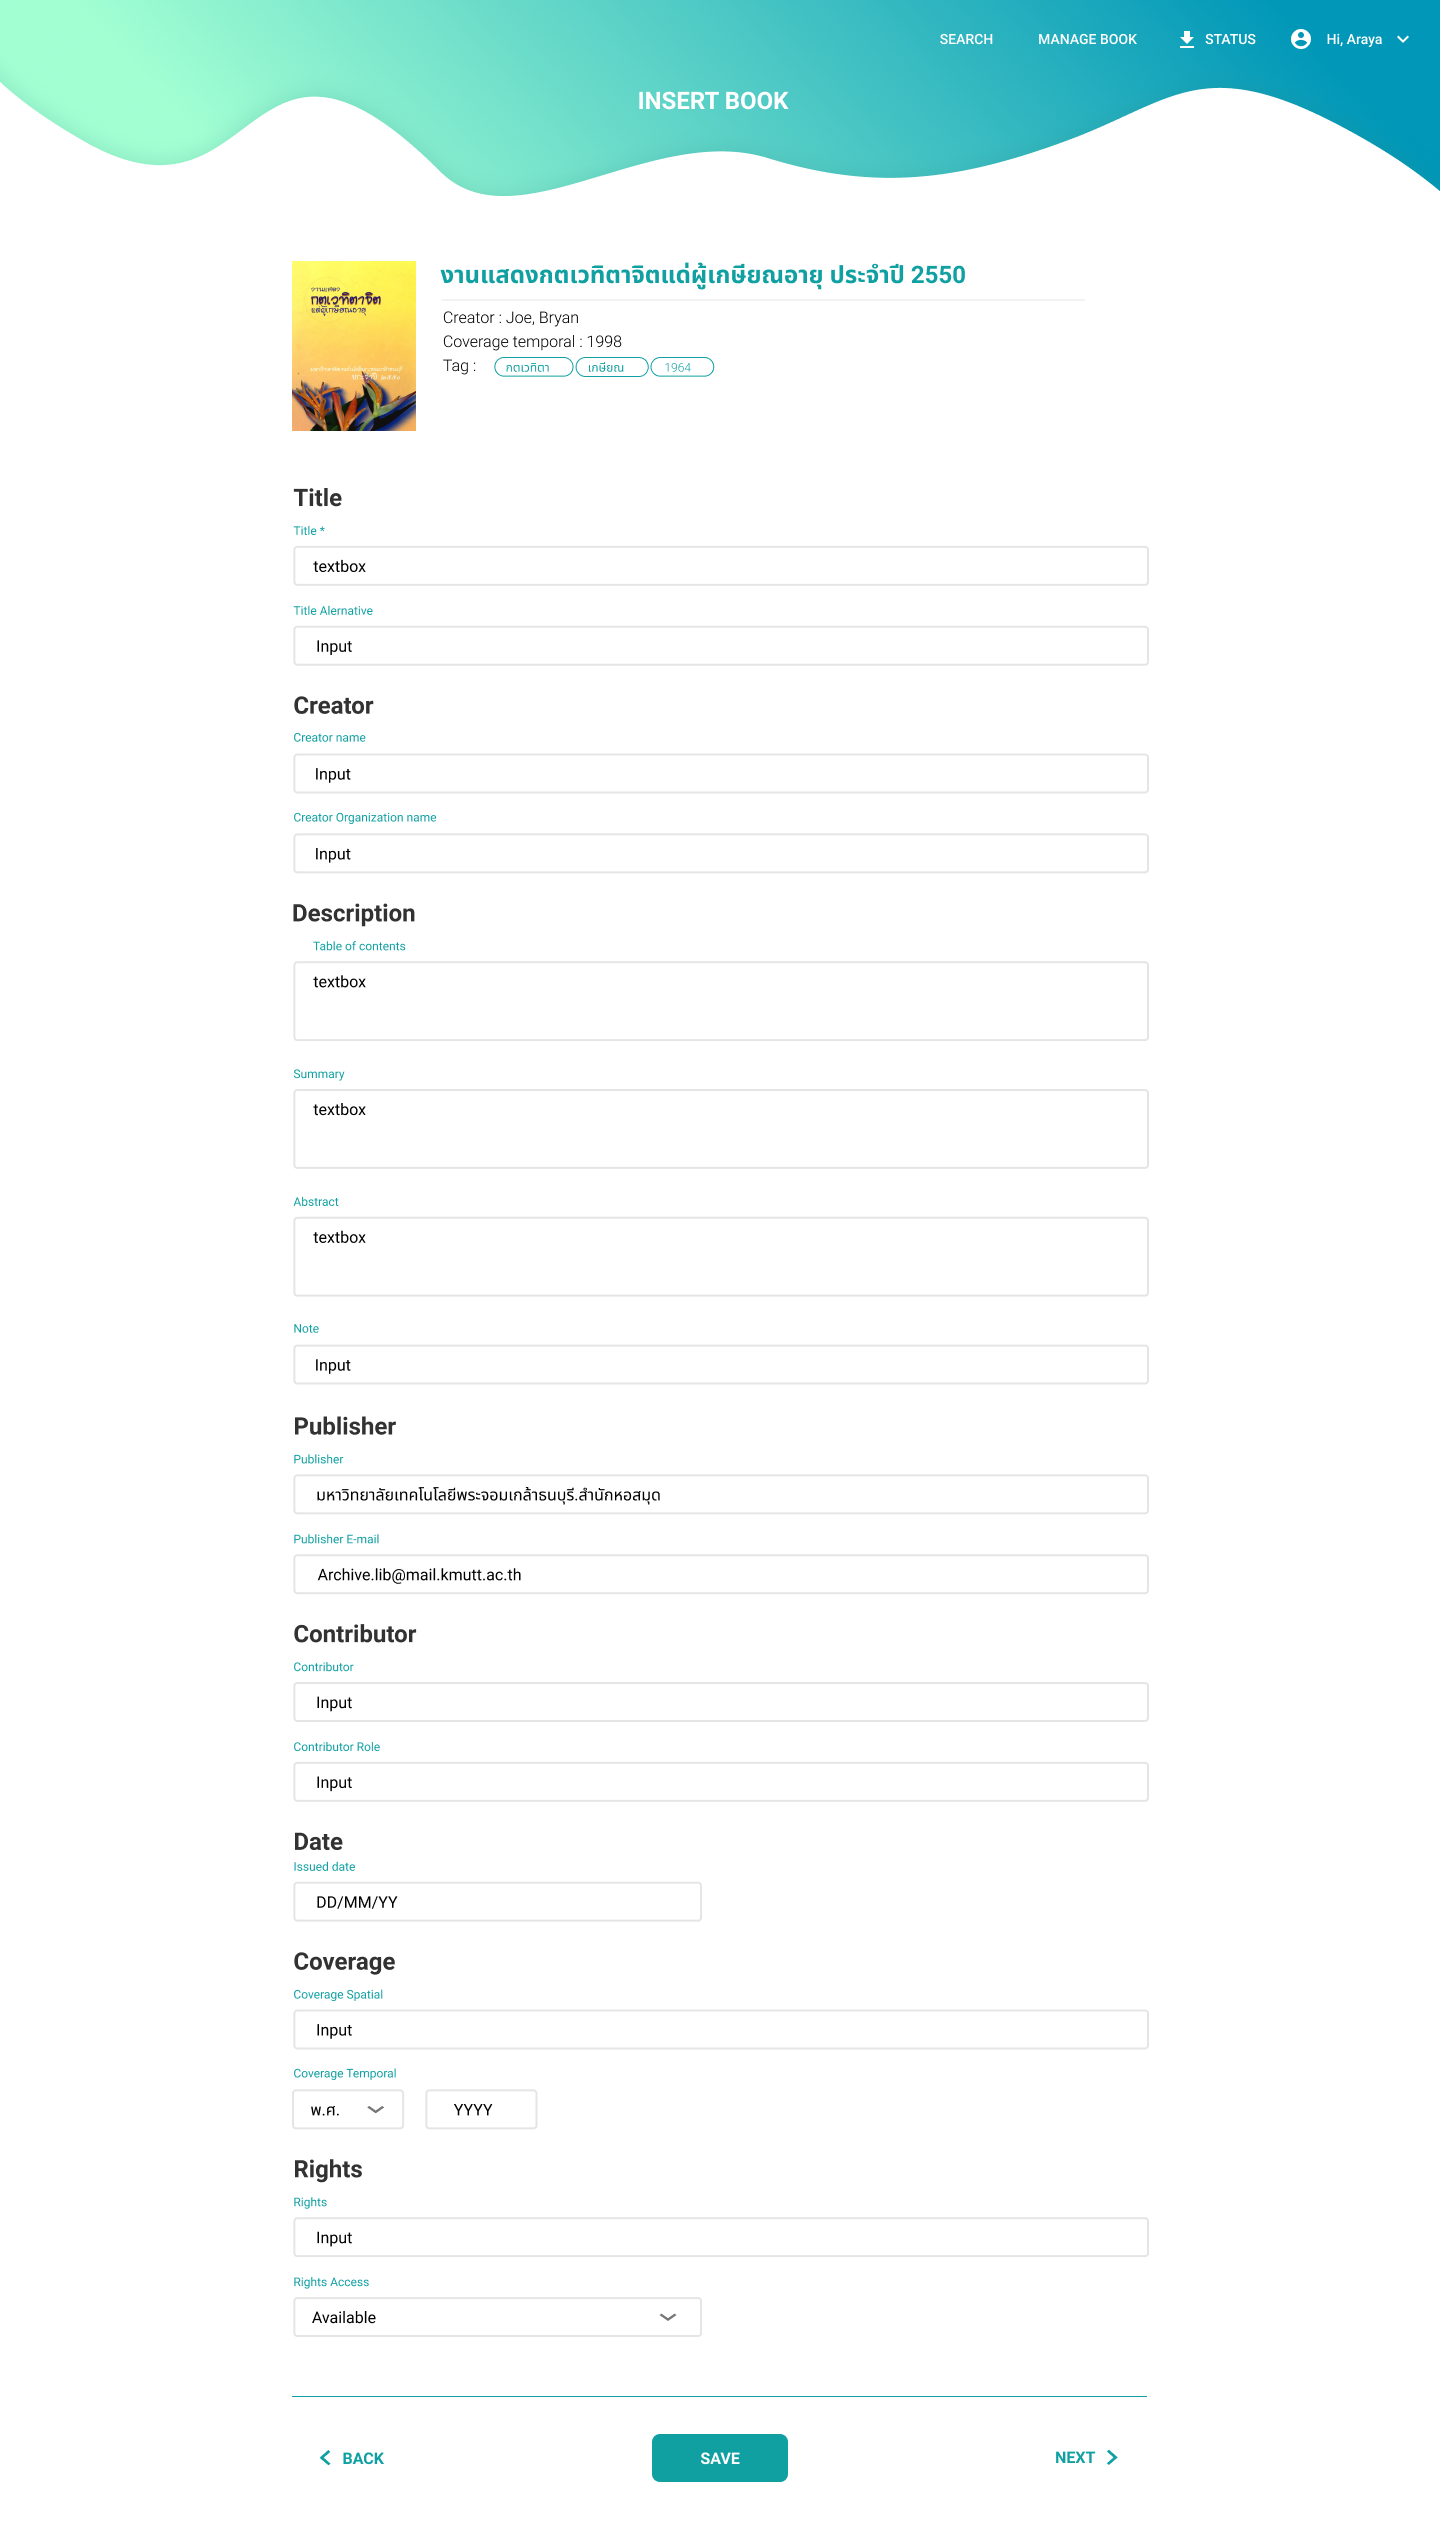
\includegraphics[scale=0.3]{e1}
    \caption{ภาพแสดงขั้นตอนการแก้ไขหนังสือขั้นที่ 1}\label{fig:e1}
\end{figure}

\begin{figure}[H]
    \centering
    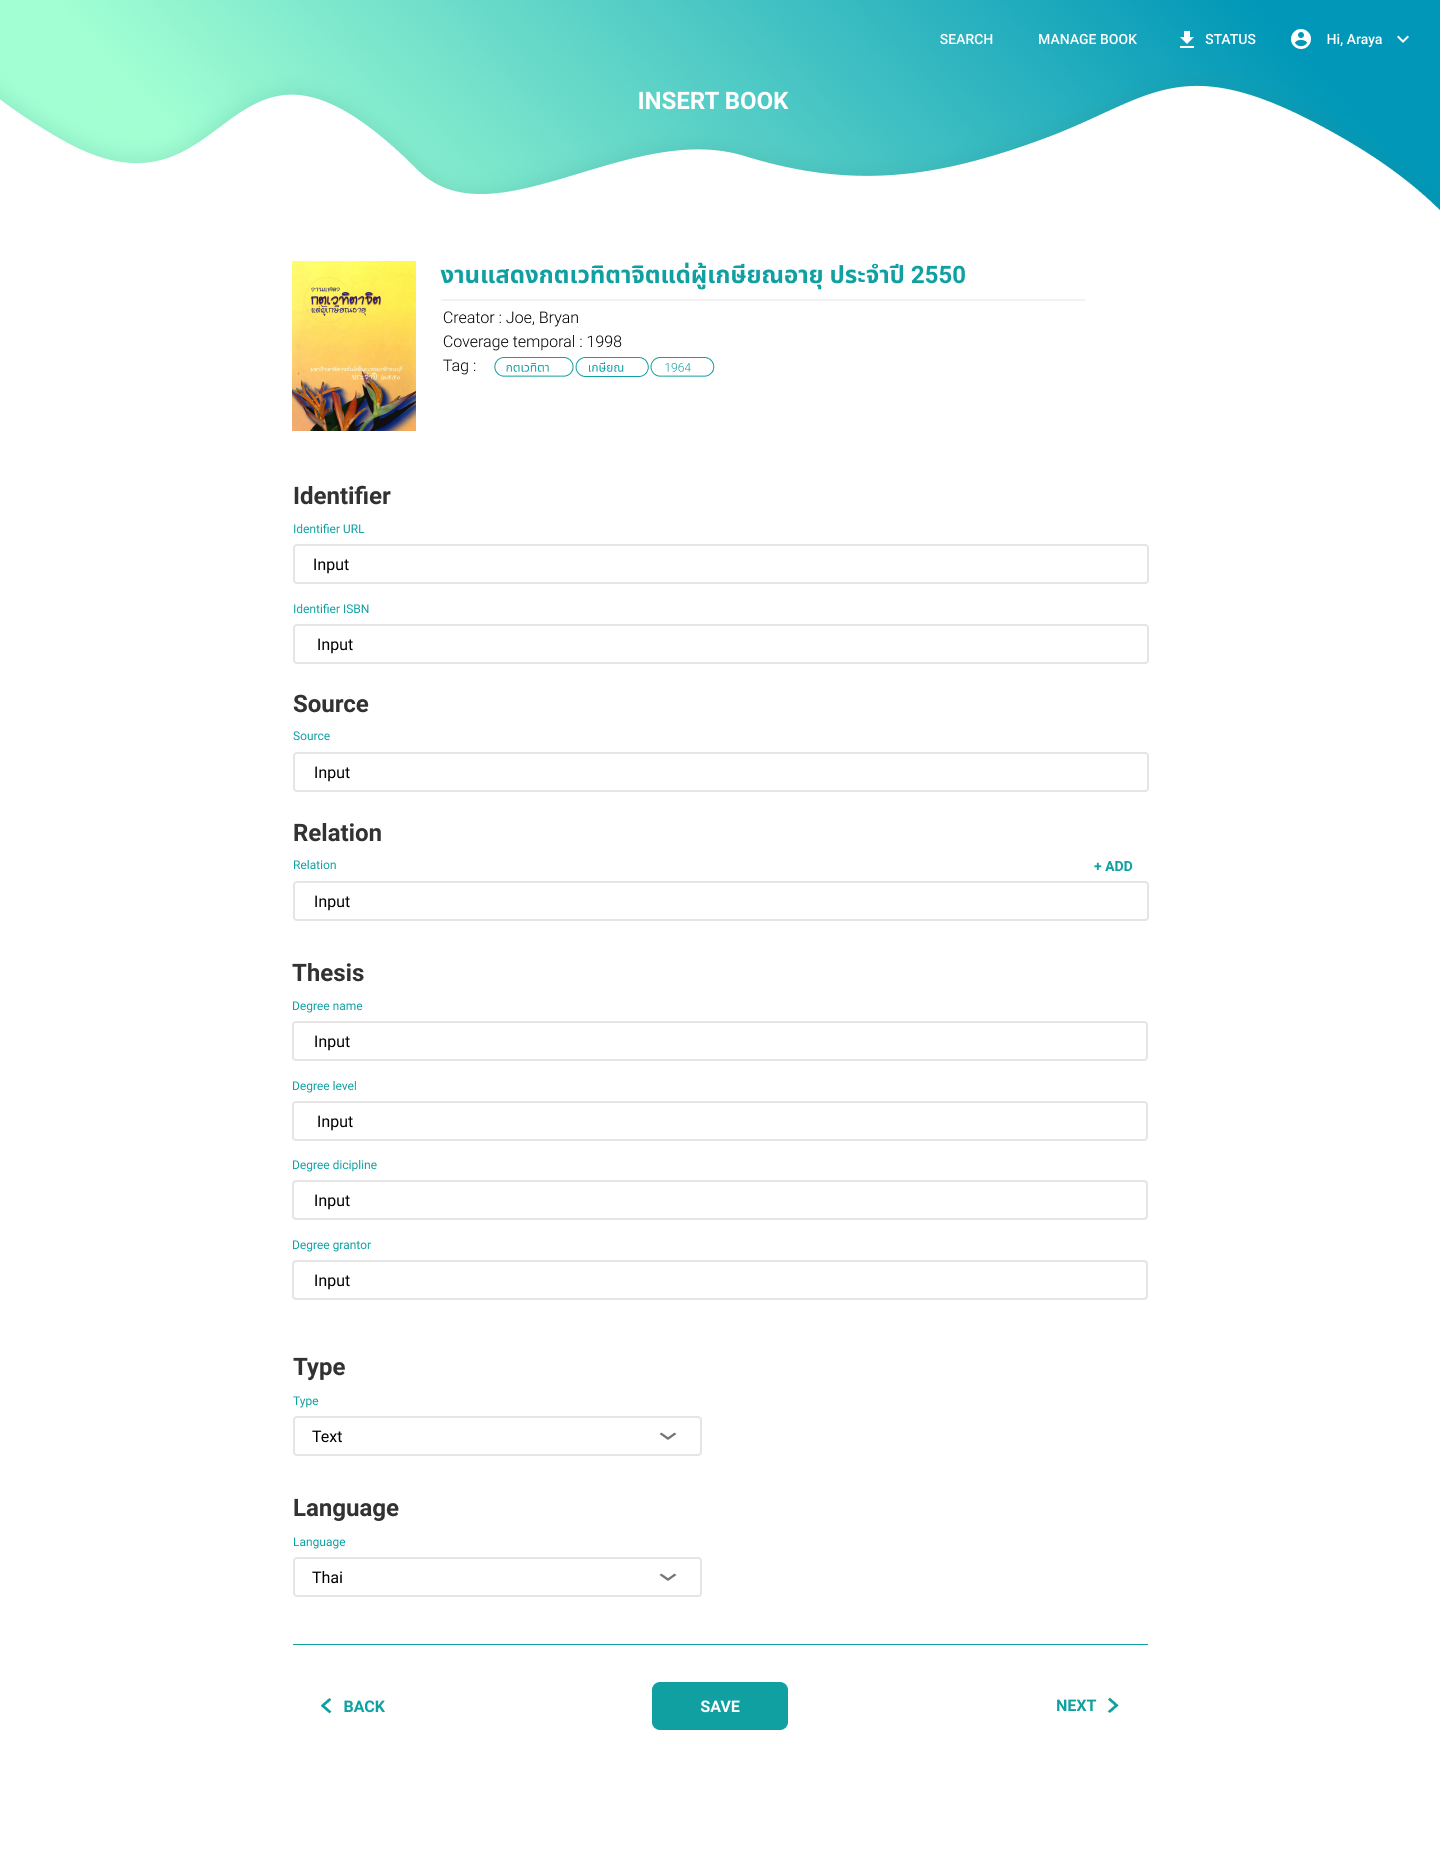
\includegraphics[scale=0.3]{e2}
    \caption{ภาพแสดงขั้นตอนการแก้ไขหนังสือขั้นที่ 2}\label{fig:e2}
\end{figure}

\begin{figure}[H]
    \centering
    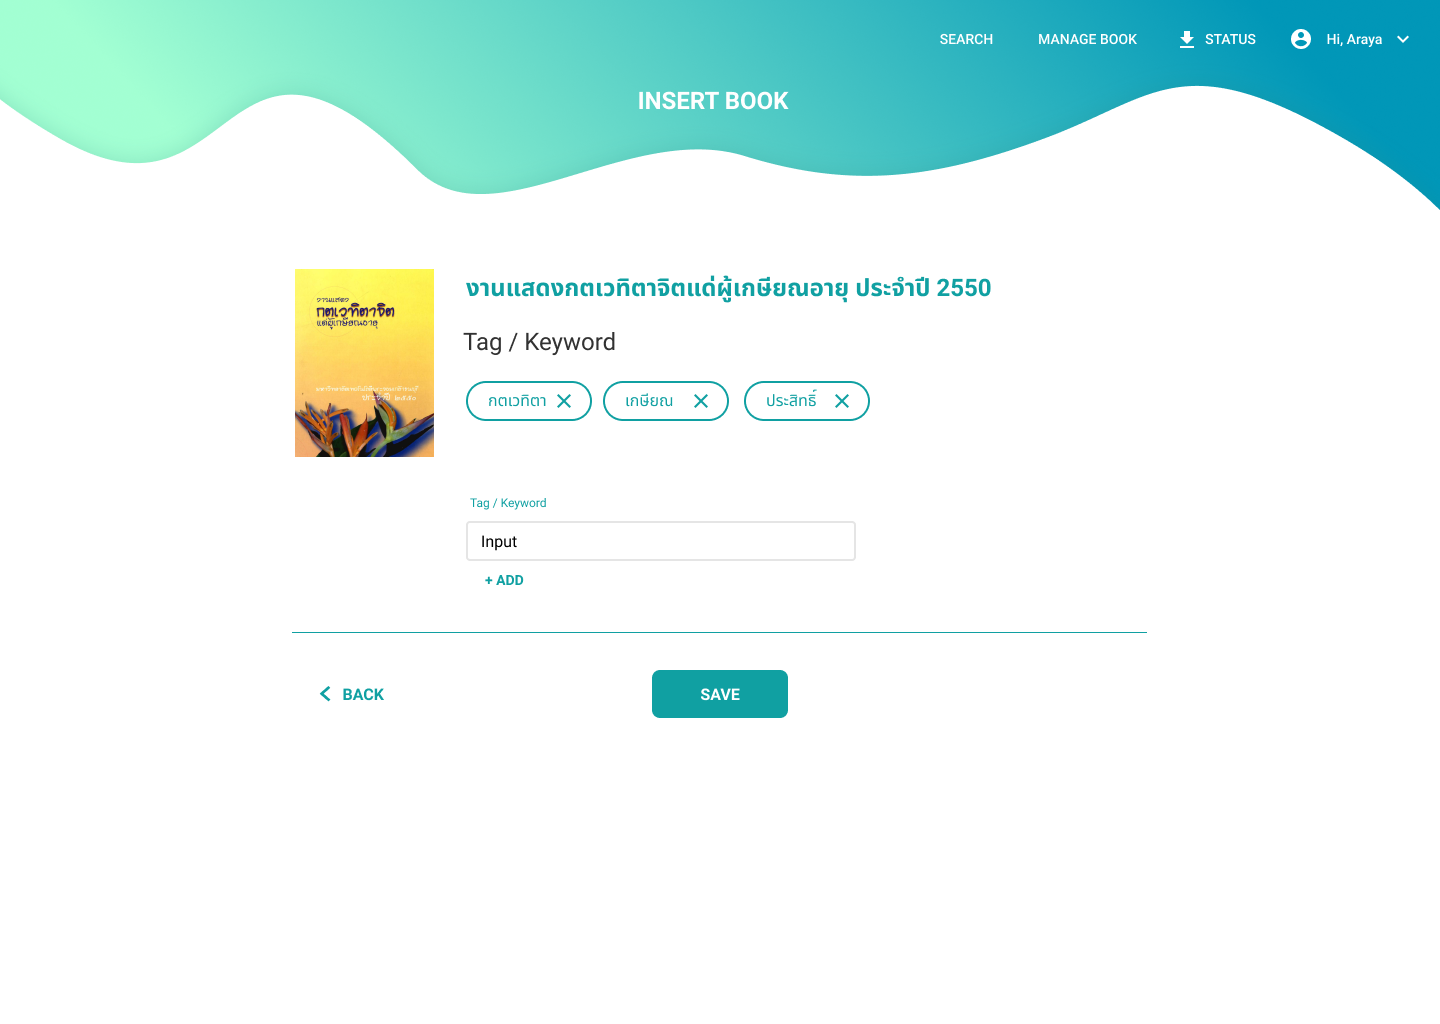
\includegraphics[scale=0.3]{e3}
    \caption{ภาพแสดงขั้นตอนการแก้ไขหนังสือขั้นที่ 3}\label{fig:e3}
\end{figure}

หน้าแก้ไขหนังสือแบ่งออกเป็น 3 ขั้นตอนดังรูป 3.35 - 3.37 ซึ่งจะมีให้แก้ไข ข้อมูลที่เคยกรอกไว้ตอนเพิ่มหนังสือเข้ามา โดยจะมีรูปปกหนังสือและชื่อหนังสือคอยบอกว่ากำลังแก้ไขหนังสือเล่มไหนอยู่ และในทุกหน้าจะมีปุ่มสำหรับบันทึกในทุกหน้าเพื่อที่จะสามารถบันทึกโดยที่ไม่ต้องรอไปหน้าสุดท้ายเพื่อบันทึกข้อมูล

\subsection{Upload Status Page}
\begin{figure}[H]
    \centering
    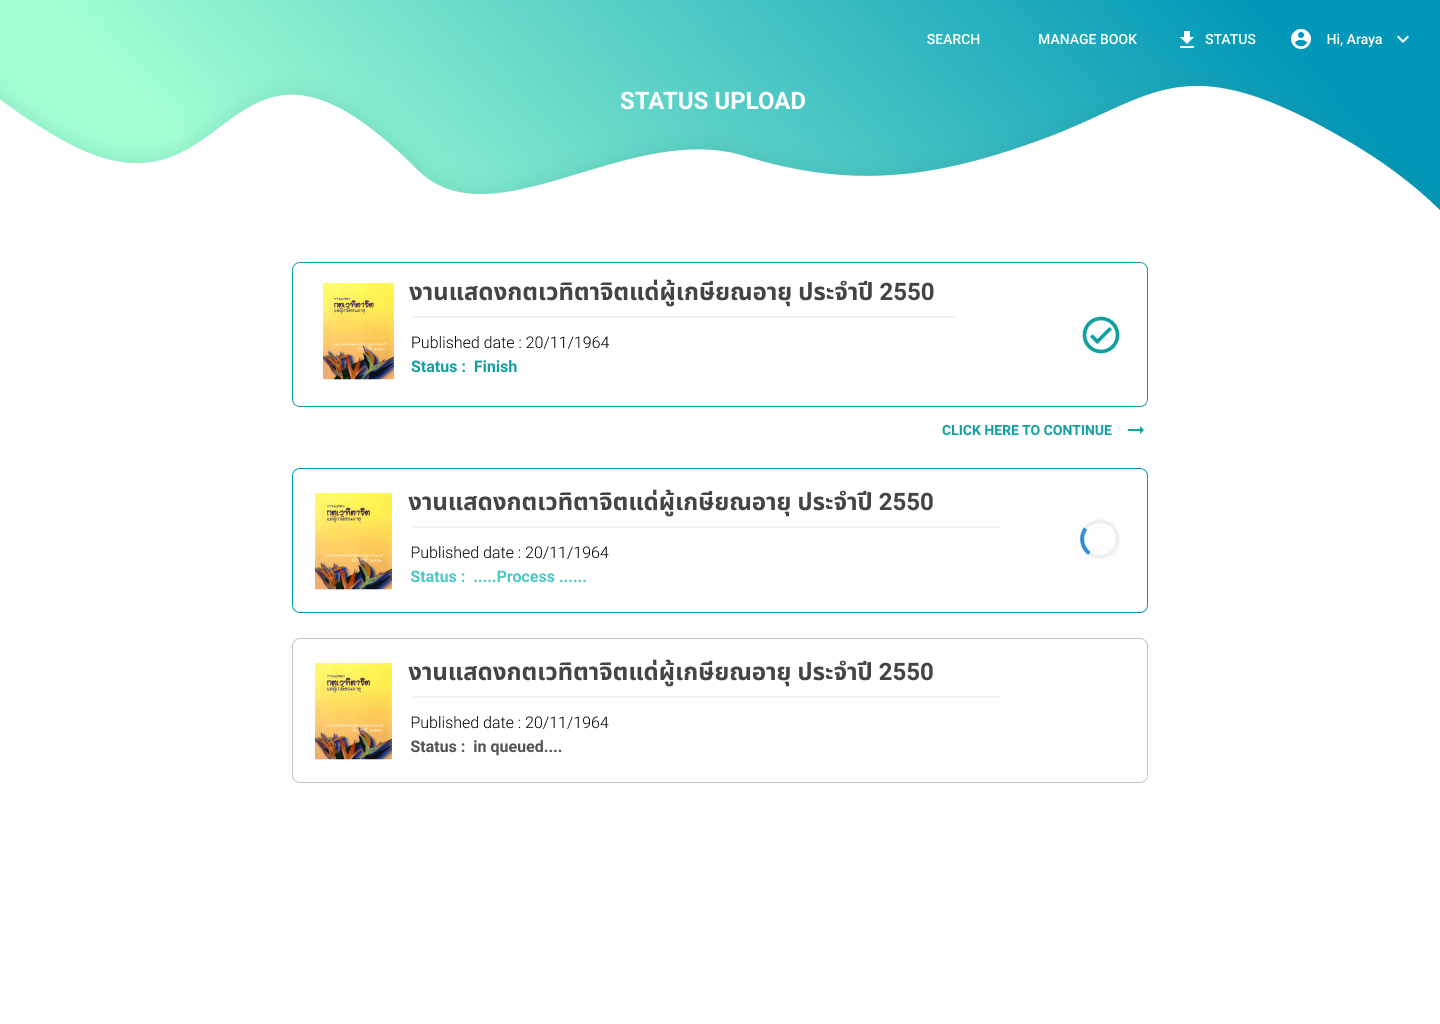
\includegraphics[scale=0.3]{status}
    \caption{ภาพแสดงหน้าการโหลดข้อมูล}\label{fig:status}
\end{figure}
จากรูป 3.38 สำหรับผู้ใช้ที่ทำการเพิ่มเอกสารเข้าสู่ระบบจะมีหน้าสำหรับโหลดกรณีที่กดออกมาหลังจากผ่านขั้นตอนการเพิ่มหนังสือขั้นตอนที่ 4 จะสามารถเข้ามาดูสถานะและทำการดำเนินการต่อได้โดยไม่ต้องผ่านการเพิ่มหนังสือเข้าสู่ระบบใหม่


\subsection{Evaluate Process Design}

ในส่วนของการประเมินผลการทำงานนั้นจะแบ่งออกเป็น 2 ส่วนคือ ส่วนของการทำ image processing จะช่วยให้การทำ OCR มีประสิทธิภาพมากเท่าไร และส่วนของระบบการค้นหา โดยในส่วนของ OCR จะทำการประเมินจากการเลือกเช็คคำจาก 2 หน้าของแต่ละเอกสารมาเช็คว่าแต่ละหน้ามีคำผิดเท่าไร โดยจะเลือกวัดเอกสารทั้งหมด 5 เล่มแบบสุ่มและเทียบการทำ Image processing ว่าทำแบบไหนได้ผลลัพธ์แบบไหนออกมา

\begin{table}[H]
\caption{ตารางประเมินการทำ OCR}\label{tbl:ocr}
\begin{tabular}{|c|c|c|c|c|}
\hline
\multicolumn{5}{|c|}{ตารางประเมินการทำ OCR}                 \\ \hline
หนังสือ & หน้า & จำนวนคำทั้งหมด & คำที่ผิด(\%) & คำเกิน(คำ) \\ \hline
        &      &                &              &            \\ \hline
\end{tabular}
\end{table}

ระบบการค้นหา จะเช็คโดยให้ผู้ใช้เป็นผู้ประเมินว่าได้รับเอกสารตรงตามที่ต้องการหรือไม่โดยจะให้เจ้าหน้าที่บรรณารักษ์คัดเลือกหนังสือจำนวน 3 เล่มที่คาดหวังว่าจะขึ้นมาเมื่อค้นหาทั้งหมด 10 ครั้ง

\begin{table}[H]
\caption{ตารางประเมินระบบการค้นหา}\label{tbl:searchtest}
\begin{tabular}{|c|l|p{0.40\linewidth}|}
\hline
\multicolumn{3}{|c|}{ตารางประเมินระบบการค้นหา}                                                                                                                                                                                                                                                                                                                                                                                                                                                                                                                                                \\ \hline
คำค้นหา                & \multicolumn{1}{c|}{หนังสือที่คาดหวัง} & \multicolumn{1}{c|}{การค้นหา}                                                                                                                                                                                                                                                                                                                                                                                                                                                                                               \\ \hline
\multicolumn{1}{|l|}{} &                                        & \makecell[l]{คะแนน 5 ระดับ\\ 5   = ค้นหาหนังสือได้ตรงตามที่ต้องการ \\และมีหนังสือที่เกี่ยวข้องกับคำค้นหาขึ้นมาอย่างถูกต้อง\\ 4   = ค้นหาหนังสือได้ถูกต้องตามที่ต้องการ\\บางเล่มและมีหนังสือที่เกี่ยวข้องกับคำค้นหาขึ้นมา\\ 3   = ไม่สามารถค้นหาหนังสือที่ต้องการแต่\\มีหนังสือที่เกี่ยวข้องกับคำค้นหาขึ้นมา\\ 2   = สามารถค้นหาหนังสือที่มีความเกี่ยวข้องกับคำค้นหา \\และมีหนังสือที่ไม่เกี่ยวข้องกับการค้นหาแสดงในผลัพธ์\\ 1 = ไม่มีหนังสือที่เกี่ยวข้องขึ้นมาในผลลัพธ์} \\ \hline
\end{tabular}
\end{table}

\begin{table}[H]
\caption{ตารางประเมิน Design}\label{tbl:design}
\begin{tabular}{|l|l|l|l|l|}
\hline
\multicolumn{5}{|c|}{ตารางประเมิน Design}                                                                                                                                                            \\ \hline
\multicolumn{1}{|c|}{\multirow{2}{*}{เกณฑ์การประเมิน}} & \multicolumn{2}{c|}{ผลลัพธ์}                             & \multicolumn{1}{c|}{\multirow{2}{*}{หมายเหตุ}} & \multicolumn{1}{c|}{คำเกิน(คำ)} \\ \cline{2-3} \cline{5-5} 
\multicolumn{1}{|c|}{}                                 & \multicolumn{1}{c|}{ผ่าน} & \multicolumn{1}{c|}{ไม่ผ่าน} & \multicolumn{1}{c|}{}                          & \multicolumn{1}{c|}{}           \\ \hline
1.หน้าเข้าสู่ระบบ                                      &                           &                              &                                                &                                 \\ \hline
2.Insert Book                                          &                           &                              &                                                &                                 \\ \hline
3.Search                                               &                           &                              &                                                &                                 \\ \hline
4.Manage Book                                          &                           &                              &                                                &                                 \\ \hline
5.View Book                                            &                           &                              &                                                &                                 \\ \hline
6.Home page                                            &                           &                              &                                                &                                 \\ \hline
7.Status Page                                          &                           &                              &                                                &                                 \\ \hline
\end{tabular}
\end{table}

\begin{table}[H]
\caption{ตารางประเมิน test}\label{tbl:test}
\begin{tabular}{|l|l|l|l|}
\hline
\multicolumn{4}{|c|}{ตารางประเมิน Test}                                                                                                                                             \\ \hline
\multicolumn{1}{|c|}{\multirow{2}{*}{เกณฑ์การประเมิน}}                  & \multicolumn{2}{c|}{ผลลัพธ์}                             & \multicolumn{1}{c|}{\multirow{2}{*}{หมายเหตุ}} \\ \cline{2-3}
\multicolumn{1}{|c|}{}                                                  & \multicolumn{1}{c|}{ผ่าน} & \multicolumn{1}{c|}{ไม่ผ่าน} & \multicolumn{1}{c|}{}                          \\ \hline
1. สามารถเข้าสู่ระบบและออกจาก ระบบได้                                   &                           &                              &                                                \\ \hline
2. สามารถเพิ่มเอกสารเข้าสู่ระบบได้                                      &                           &                              &                                                \\ \hline
3. สามารถแก้ไขรายละเอียดเอกสารที่อยู่ในระบบได้                          &                           &                              &                                                \\ \hline
4.   สามารถตรวจสอบและแก้ไขคำที่เพิ่มเข้ามาในระบบในขั้นตอนเพิ่มเอกสารได้ &                           &                              &                                                \\ \hline
5. สามารถลบเอกสารที่อยู่ในระบบได้                                       &                           &                              &                                                \\ \hline
6.   สามารถค้นหาข้อมูลเอกสารภายในระบบได้                                &                           &                              &                                                \\ \hline
7.   สามารถเรียกดูเอกสารที่ต้องการได้                                   &                           &                              &                                                \\ \hline
\end{tabular}
\end{table}